\documentclass[13pt, a4paper]{extarticle}

\usepackage{../packages_tex}
\tcbuselibrary{minted,skins,breakable,theorems}
\usemintedstyle{pastie}
% begin pythoncode
\newtcblisting[auto counter, list inside=py]{pythoncode}[3][]{
  listing engine=minted,
  listing only,
  breakable,
  nobeforeafter,
  minted style=pastie,
  minted language=python,
  minted options={numbersep=3mm,texcl=true,#1},
  left=5mm,enhanced,
  title={\bf Script \thetcbcounter}: #3,
  #2
}
% end pythoncode
\newcommand{\blue}[1]{\textcolor{blue}{#1}}
\newcommand{\red}[1]{\textcolor{red}{#1}}

\newcommand{\update}[1]{{\color{ForestGreen} #1}}
\newcommand\ideas[1]{\emph{\ul{Id\'ees}: {#1}}}
\newcommand\refs[1]{{\bf \ul{Biblio}}: #1}
\newcommand\todo[1]{{\color{red} \Large (#1)}}
\usepackage{appendix}
\renewcommand{\appendixpagename}{Annexes}
\renewcommand{\appendixtocname}{Annexes}
\captionsetup{justification=centering}
\tcbuselibrary{theorems}
\captionsetup[figure]{labelfont={bf},name={Fig.},labelsep=period}
\captionsetup[table]{labelfont={bf},name={Table},labelsep=period}

\newcommand{\filt}[1]{\overline{#1}^\ell}
\usepackage[colorlinks,bookmarks=false,citecolor=blue,linkcolor=blue,urlcolor=blue]{hyperref}

\addto\captionsenglish{
  \renewcommand{\contentsname}%
    {Table des matières}}%
\addto\captionsenglish{\renewcommand{\refname}{Références}}

\begin{document}
    
\begin{titlepage}
    \begin{center}
  
        {\Huge Rapport de stage}
        
        \vspace{0.2cm}
   
              \centering
        {\huge \bf Analyse statistique d'un écoulement turbulent}
        
        \vspace{2cm}
        \centering
        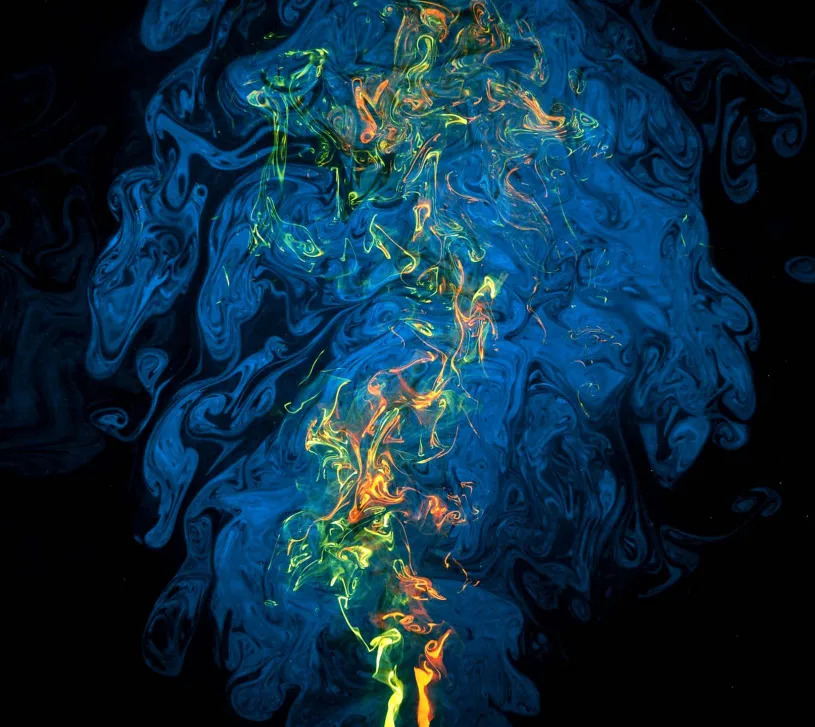
\includegraphics[width=14cm]{figs/turb.jpg}

             \vspace{1.5cm}
              {\huge ALLAGLO Nikita} \\
             
              \vspace{3cm}
 
        {\huge L3 Physique}\\
          \centering
          
\includegraphics[width=0.2\textwidth]{figs/logo_PS.jpg} 
          
\includegraphics[width=0.2\textwidth]{figs/logo_lisn.png}
              \vspace{1cm}
             
        {\large Le 14 juillet 2023}
  
    \end{center}
 \end{titlepage}

\pagenumbering{roman}

\tableofcontents
\newpage
\listoffigures
\listoftables
\tcblistof[\section*]{py}{Liste des scripts}

\newpage
\pagenumbering{arabic}

\setstretch{1.1}

\section{Introduction}
\noindent La turbulence est une branche de recherche en pleine activité en mécanique 
des fluides. Expérimentée au quotidien dans une fumée de cigarette par exemple, du fait 
de son origine hautement non-linéaire, elle demeure un casse-tête auquel se heurtent 
et physiciens et mathématiciens. Dans une ère où les théories statistiques sont 
omniprésentes en recherche fondamentale, l'approche la plus rapide permettant de mieux 
éclairer les {\it{voies sombres de la turbulence}} est précisément de passer par 
l'analyse statistique. En couplant ainsi ces méthodes statistiques à des théories 
novatrices de transferts inter-échelles \cite{Dubrulle-Beyond}, on aboutit à un 
cadre de travail idéal pouvant potentiellement démêler les phénomènes complexes 
intrinsèques aux équations régissant la mécanique des fluides. Le présent stage 
s'est en conséquence articulé autour de trois axes majeurs: dans un premier 
temps, nous avons saisi les rudiments de la théorie, en partant des idées 
phénoménologiques de Kolmogorov pour parvenir aux liens entre turbulence et 
irrégularité du champ de vitesse.
Dans un second temps, assisté par les infrastructures de calcul haute performance 
offertes par le \emph{Laboratoire Interdisciplinaire des Sciences du Numérique} où 
nous avons effectué notre stage, nous avons développé un module de traitement 
des données permettant d'analyser efficacement des bases de données d'écoulement 
turbulent de l'ordre du TeraByte. En dernier lieu, à l'aide de ce module, nous 
avons pu mettre en évidence quelques inexactitudes hypothétisées dans les résultats 
décrits dans un article écrit par l'équipe encadrante \cite{Faller-Intermittency} 
(issu de la thèse d'un ancien doctorant).

\section{Contexte}

\subsection{Turbulence hydrodynamique}

\subsubsection{Nombre de Reynolds}

\noindent La turbulence est un régime d'écoulement caractérisé par un champ de vitesse chaotique.
Quiconque n'a jamais pris l'avion a probablement déjà expérimenté le phénomène. Bien que les 
équations régissant le mouvement des fluides soient déterministes, un écoulement turbulent possède
une très forte sensibilité aux conditions initiales - ce qui rend le système quasi-imprédictible à
temps long. On sait qu'il existe encore des résultats non démontrés à ce jour en mécanique 
des fluides (cf. problème d'existence et de régularité des solutions des équations de Navier-Stokes
de l'Institut Clay) et la recherche en turbulence n'échappe pas à cette loi: Richard Feynman est 
allé jusqu'à qualifier la turbulence comme le plus important problème non-résolu de la physique 
classique. On s'attend naturellement à ce que, face à un état si complexe, on puisse chercher à 
catégoriser les écoulements par leur nature turbulente ou non. Un paramètre de contrôle existe à 
ce propos: \emph{le nombre de Reynolds} qui prend forme en considérant les équations de Navier-
Stokes adimensionnées. Pour un fluide incompressible, nous avons :
\begin{align}
    \del_t u_i + u_j\del_ju_i &= -\dfrac{1}{\rho}\del_i p + \nu\del_j\del_ju_i + f_i\label{eq:NS}\\
    \del_i u_i &= 0,
\end{align}
où $\git{u}$ est la vitesse du fluide, $\rho$ sa densité de masse, $p$ la pression, $\nu$ la 
viscosité cinématique et $f$ la résultante des forces externes. En incorporant la longueur 
caractéristique $L$ et vitesse caractéristique $U$ de l'écoulement de telle sorte que 
$\del_i= \frac{1}{L}\del'_i$, $u_i=Uu'_i$, $p=\rho U^2p'$\footnote{une pression est une énergie par unité de volume} 
et $\del_t = \frac{U}{L}\del'_t$, on obtient (pour Navier-Stokes):
\begin{align}
     &\frac{U^2}{L}\del'_t u'_i + \frac{U^2}{L}u'_j\del'_ju'_i = -\frac{U^2}{L}\del'_ip' + 
     \nu \frac{U}{L^2}\del'_j\del'_ju'_i + f_i \\
     \Rightarrow~&\del'_t u'_i + u'_j\del'_ju'_i = -\del'_i p' + \dfrac{1}{\text{Re}}\del'_j\del'_ju'_i 
     + \frac{L}{U^2}f_i
\end{align}
avec Re le nombre de Reynolds défini comme
\begin{align}
    \boxed{\text{Re} = \dfrac{UL}{\nu} \sim \dfrac{|(u\cdot\grad) u|_\text{caract.}}{|\nu\grad^2u|_\text{caract.}}}.
\end{align}
Lorsque $\text{Re}\ll 1$, l'équation devient quasi-linéaire puisque le terme en laplacien domine.
Dans ce cas, on retrouve un semblant d'équation de diffusion $\pdv{X}{t} \sim \nu\pdv[2]{X}{t}$, 
on comprend alors bien que la viscosité 
agit comme un agent {\bf diffusif}; il est impossible qu'il y ait apparition de tourbillons dans
l'écoulement.
Dans le cas où $\text{Re}\gg 1$, le terme non-linéaire est dominant. On peut alors montrer que si, 
avec certaines conditions initiales, l'écoulement était parallèle pour $\text{Re}\ll 1$, il y a 
plutôt apparition de tourbillons à différentes échelles pour $\text{Re}\gg 1$ et donc un chaos 
progressif. La dérivée particulaire permet de comprendre ce phénomène: c'est la vitesse elle-même
qui "se transporte" d'où la non-linéarité.
C'est ce caractère alors qui mène au chaos par sensibilité locale. Nous verrons dans la section \S
\ref{sec:cascade} suivante que c'est précisément une hiérarchie d'échelles qui permet de 
comprendre - avec les mains - le concept de turbulence.

\subsubsection{Cascade turbulente}\label{sec:cascade}
\begin{figure}[h]
    \centering
    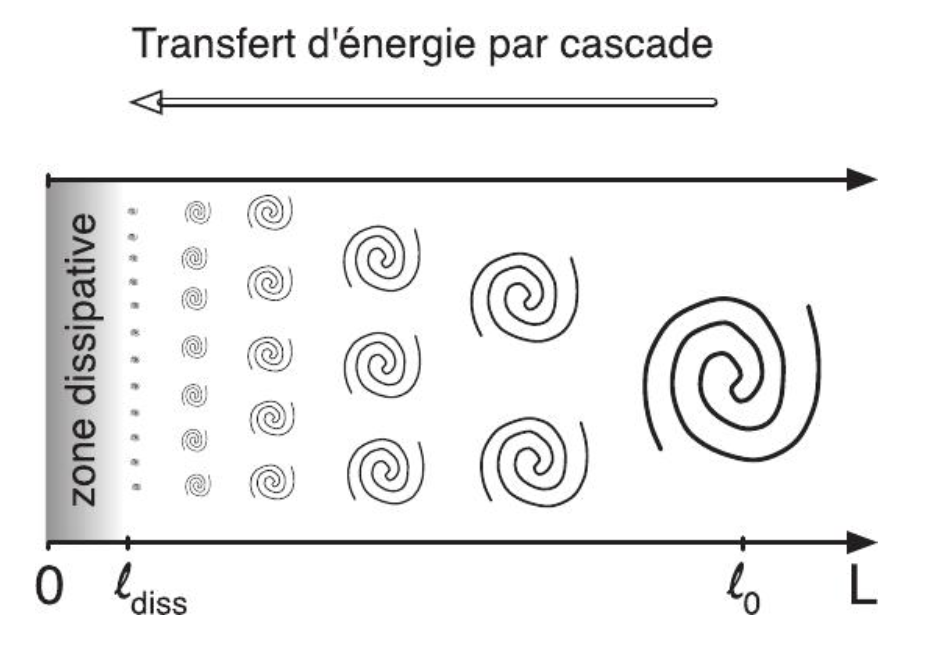
\includegraphics[width=.9\linewidth]{figs/cascade_tourbillons.png}
    \caption[La turbulence vue comme une cascade de tourbillons des grandes vers les petites échelles]
    {La turbulence vue comme une cascade de tourbillons des grandes vers les petites échelles. 
    $\ell_\text{diss}\ll\ell\ll\ell_0$ représente la zone inertielle. Figure reprise de \cite{Galtier-Turb}.}
    \label{fig:cascade_tourb}
\end{figure}
\noindent La turbulence peut être comprise par des arguments phénoménologiques. Lewis Fry 
Richardson fut le premier à mettre en évidence ce que l'on nomme aujourd'hui la \emph{cascade 
turbulente} sous les vers suivants:
\begin{center}
    \emph{Big whirls have little whirls that feed on their velocity},\\
    \emph{and little whirls have lesser whirls and so on to viscosity}.
\end{center}
Comme le schématise la figure \ref{fig:cascade_tourb}, il existe une cascade énergétique 
permettant le transfert d'énergie des gros tourbillons aux plus petits - à condition d'être dans 
une échelle suffisamment grande pour que la viscosité ne puisse pas encore dissiper et 
suffisamment petite pour être aveugle aux phénomènes à grande échelle (l'injection d'énergie dans
le système par exemple): on parle de \emph{zone intertielle}. C'est ainsi dans cette zone que la 
physique non-linéaire demeure influente. Dans la suite de ce rapport, la limite inférieure des 
échelles de la zone inertielle sera appelée \emph{échelle de Kolmogorov} et notée $\eta$. L'idée de
cascade de tourbillons repose en toute rigueur sur une vision très simplifiée puisque, dans la 
réalité, on observe plutôt des tubes de vorticité imbriqués les uns dans les autres\cite{Galtier-Turb}.
Kolmogorov a développé une série d'articles dans le courant des années 1940 permettant d'appuyer 
cette idée de cascade de turbulence \cite{K41}.
Il a notamment obtenu des lois universelles (indépendantes de la viscosité) {\bf valables sur 
toute la zone inertielle} pour une \ul{turbulence statistiquement homog\`ene et isotrope} 
vérifiées par l'expérience: on a en idée les densités spectrales d'énergie qui affichent une 
dépendance en $k^{-5/3}$ sur la zone inertielle. Même s'il existe toute une théorie permettant de
démontrer cela dans le cas d'une turbulence statistiquement homogène et isotrope, on peut obtenir
ce résultat par simple analyse dimensionnelle. Nous avons vu comment, à partir de modèles jouets, on
pouvait aboutir à certaines propriétés remarquables de turbulence. Il s'agit désormais de pouvoir
généraliser à une turbulence non homogène et anisotrope, pouvant expliquer des propriétés émergentes du chaos comme 
l'intermittence mais surtout pouvant capter des singularités.

\subsubsection{Dissipation anormale}\label{sec:anomalous}

\noindent La question de la régularité/des singularités est une branche de recherche très 
active en mécanique des fluides (il suffit de penser au prix de l'Institut Clay). Le problème 
se pose notamment lorsque l'on prend en considération la \emph{0ème loi de la turbulence}. 
\begin{tcolorbox}[colback=Goldenrod,title={Zéroième loi de la turbulence}]
		La puissance injectée moyenne (ou le taux moyen de variation de l'énergie cinétique) au sein 
    d'un fluide tend vers une constante non-nulle à viscosité rigoureusement nulle.
\end{tcolorbox}
\noindent On parle d'anomalie dissipative (ou de dissipation anormale) car la viscosité est 
(normalement) la seule grandeur pouvant dissiper de l'énergie: s'il n'existe rien qui se 
"nourrit" de l'énergie injectée, comment expliquer un taux moyen de dissipation non-nul ? 
Cela suggère l'existence d'un autre mécanisme intervenant dans les écoulements très 
turbulents ($\text{Re}\to\infty$). 
À partir des équations de Navier-Stokes, on peut démontrer l'expression \ul{exacte} 
du taux moyen de dissipation dans un fluide \cite{Galtier-Turb}:
\begin{align}
    \displaystyle\pdv{\mean{E}}{t} = \rho\nu\mean{\omega^2},
\end{align}
avec $\mean{E}$ l'énergie cinétique moyenne par unité de volume et 
$\git{\omega}=\rot{\git{u}}$ la vorticité. Si $\nu\to 0$, la 0ème loi de la turbulence 
implique que $\mean{\omega^2}\to\infty$. Un rotationnel infini provient d'un champ de
 vitesse irrégulier. Les irrégularités seraient alors responsables de l'anomalie dissipative: 
 c'est la conjecture d'Onsager. On comprend alors tout l'intérêt de développer une 
 théorie incorporant de façon fondamentale le caractère singulier des grandeurs 
 physiques comme la vitesse ou la vorticité. \\
Cette théorie est basée sur une formulation faible des équations décrivant les fluides 
prenant précisément en compte ce qui est \emph{non-lisse} \cite{Dubrulle-Beyond, DuchonRobert}.
On s'attend bien à rencontrer des concepts inhérents à la théorie des distributions, 
les fonctions-test en particulier 
seront vitales dans cette formulation faible. Les fonctions-test seront définies comme 
les $\varphi>0\in\mathscr{C}^
\infty$ à support compact dans $\mathbb{R}^3$ et s'intégrant à l'unité. On peut 
démontrer alors que, pour $\ell$ réel,
$\varphi_\ell(\git{\xi}) := \dfrac{1}{\ell^3}\varphi\qty(\dfrac{\git{\xi}}{\ell})$ 
converge (au sens des distributions) vers un delta de Dirac. On comprend alors que 
le principal but de ces fonctions est de lisser les quantités irrégulières par une 
opération de convolution. Pour une échelle $\ell$, on définit pour un champ 
(scalaire ou vectoriel) $X$ sa version \emph{filtrée} comme:
\begin{align}
    \filt{X}(\git{r}) = \mathlarger{\int_{\mathbb{R}^3}}\varphi_\ell(\git{\xi})
    X(\git{\xi}+\git{r})\dd^3\git{\xi}
    \label{eq:filtrage}
\end{align}
Ces outils permettent alors de caractériser les transferts d'énergie inter-échelle: 
on applique tout d'abord l'opération~\eqref{eq:filtrage} aux équations de Navier-Stokes 
puis on prend le produit scalaire du résultat obtenu avec la quantité 
$\rho\frac{\git{u}}{2}$. Dans un second temps, on prend le produit scalaire de 
$\rho\frac{\filt{\git{u}}}{2}$ avec les équations de Navier-Stokes non 
filtrées~\eqref{eq:NS}. En sommant les deux résultats, on obtient l'équation 
d'évolution de l'énergie cinétique pseudo-filtrée 
$\tilde{E}_\ell:=\rho\frac{\git{u}\cdot\filt{\git{u}}}{2}$ \cite{Creff_2023}: 
\begin{align}
    \boxed{\del_t \tilde{E}_\ell + \div{\git{J}^{\text{NS}}_\ell} + 
    \mathscr{D}^\nu_\ell + \mathscr{D}^{u}_\ell
    = \mathcal{P}_\ell},
    \label{eq:filt_Kin_energy}
\end{align}
avec la définition suivante des termes de dissipation:
\begin{align}
    \git{J}^{\text{NS}}_\ell &=  \frac{\rho}{2}( (\git{u}\cdot\filt{\git{u}})\git{u} 
    - \nu \grad (\git{u}\cdot\filt{\git{u}}) + \frac{1}{2}(\filt{\git{u}} p + 
    \git{u} \filt{p}), \\ 
    \mathcal{P}_\ell &=   \frac{\rho}{2} (\git{u} \cdot \filt{\git{f}} + 
    \filt{\git{u}} \cdot \git{f} ), \\
    \mathscr{D}^\nu_\ell &=  \rho \nu \del_i \filt{u_j} \del_i u_j,  \\
    \mathscr{D}^{u}_\ell &=   \frac{\rho}{2} (\git{u}\cdot  \filt{u_i  \del_i \git{u}}
     -  u_i\git{u}\cdot \del_i \filt{\git{u}}).\label{eq:Du}
\end{align}
Tous les termes de l'équation~\eqref{eq:filt_Kin_energy} mesurent les transferts 
entre l'échelle $\ell$ et toutes les échelles hiérarchiquement supérieures. 
$\git{J}^{\text{NS}}_\ell$ est un courant de déplacement d'énergie (du fait de la 
divergence); il n'est donc pas vraiment intéressant pour tout ce qui a trait à la 
dissipation. $\mathscr{D}^\nu_\ell$ est la dissipation visqueuse. 
$\mathscr{D}^{u}_\ell$ est la dissipation anormale:
ce terme ne disparaît pas dans la limite des échelles infinitésimales \cite{DuchonRobert}. 
Notez toutefois que cette dérivation est très récente: à la place de $\mathscr{D}^{u}_\ell$,
on considère plutôt dans la littérature la dissipation inertielle notée $\mathscr{D}^I$
ou $\mathscr{D}^{\text{DR}}$. Ces dernières sont reliées par un terme de divergence:
\begin{align}
  \mathscr{D}^I_\ell = \dfrac{\rho}{2}\grad\cdot\qty(\git{u}\filt{u^2}-\filt{u^2\git{u}}) 
  + \mathscr{D}^u_\ell
  \label{eq:DI}
\end{align}
Nous expliquons en section \S \ref{sec:problematique} les raisons d'un tel changement. \\
Avant de mentionner ce que nous faisons explicitement avec toute cette théorie, 
il est bon de rappeler l'essence aléatoire de l'écoulement turbulent. On ne peut 
pas juste étudier les champs d'intérêt du point de vue de l'espace ou du temps; 
il est nettement plus pertinent de traiter l'ensemble du point de vue statistique.

\subsubsection{Traitement statistique}\label{sec:outil_turb}
\noindent Il faut imaginer reproduire la même expérience $N$ fois, au lieu de 
considérer une grandeur $X(\git{r},t)$, on considère plutôt la moyenne d'ensemble 
des $N$ réalisations $\{X_i(\git{r},t)\}_i$:
\begin{align}
    \mean{X(\git{r},t)}_N = \dfrac{1}{N}\sum_i X_i(\git{r},t).
\end{align}
Du point de vue numérique, en raison du coût des ressources computationnelles, 
on ne relance évidemment pas la même simulation $N$ fois, on propage plutôt 
temporellement les solutions des équations de Navier-Stokes, et on dispose alors 
d'un ensemble de \emph{snapshots} ("photo instantanée") prises à intervalles de 
temps très rapprochés. En théorie des systèmes dynamiques, on peut alors montrer 
qu'en attendant plus longtemps qu'un temps appelé \emph{temps de corrélation}, 
on aboutit à une configuration qui n'a plus vraiment de lien avec la condition 
initiale. On peut alors considérer $N$ expériences "répétées" comme $N$ snapshots 
suffisamment espacées temporellement. \\

\noindent Par ailleurs, plutôt que de chercher à savoir si un champ prend une 
valeur particulière, il est plus pertinent de considérer la {\bf probabilité} 
qu'il prenne cette valeur particulière. Dans ce cas, la position et le temps ne 
nous intéressent plus vraiment, ces derniers deviennent eux-mêmes en quelque 
sorte des "expériences" aléatoires. Le volume complet représente 
donc déjà un espace d'intérêt pour les statistiques {\bf spatiales}. Cet espace 
concaténé avec lui-même autant de fois qu'il y a de snapshots
devient {\bf l'espace des expériences aléatoires}: à cet espace, on peut associer
des statistiques {\bf d'ensemble}. Chaque champ
peut ensuite prendre des valeurs qui lui sont propres \underline{pour chaque expérience 
aléatoire}: il y a autant de champs que d'{\bf espaces des réalisations}. On 
insiste grandement durant ce stage sur le concept de densités de probabilité 
jointe: il s'agit de la densité de probabilité d'avoir 2 évènements simultanément.\\

\noindent Dans la présente section, nous avons introduit le contexte de travail 
théorique très général qu'est celui de la turbulence. Le stage que j'ai effectué 
ayant été avant tout numérique, nous expliciterons désormais l'écoulement considéré 
ainsi que le cadre du traitement de données.

\subsection{Géométrie et simulations numériques}
\subsubsection{Géométrie de von Kármán}
\noindent Nous considérons dans ce stage une turbulence dans une géométrie de von Kármán.
L'écoulement est généré dans un cylindre de rayon $R$ par deux turbines tournant
en sens opposés à fréquence angulaire égale. Deux configurations sont d'intérêt: 
\emph{CONTRA} et \emph{ANTI-CONTRA}
représentées respectivement par le signe + et - sur la figure \ref{fig:geo_vk}.
L'écoulement est réputé pour sa turbulence fortement inhomogène et anisotrope.
Il représente une expérience majeure pour les nouvelles théories de turbulence.
\begin{figure}[h]
  \centering
  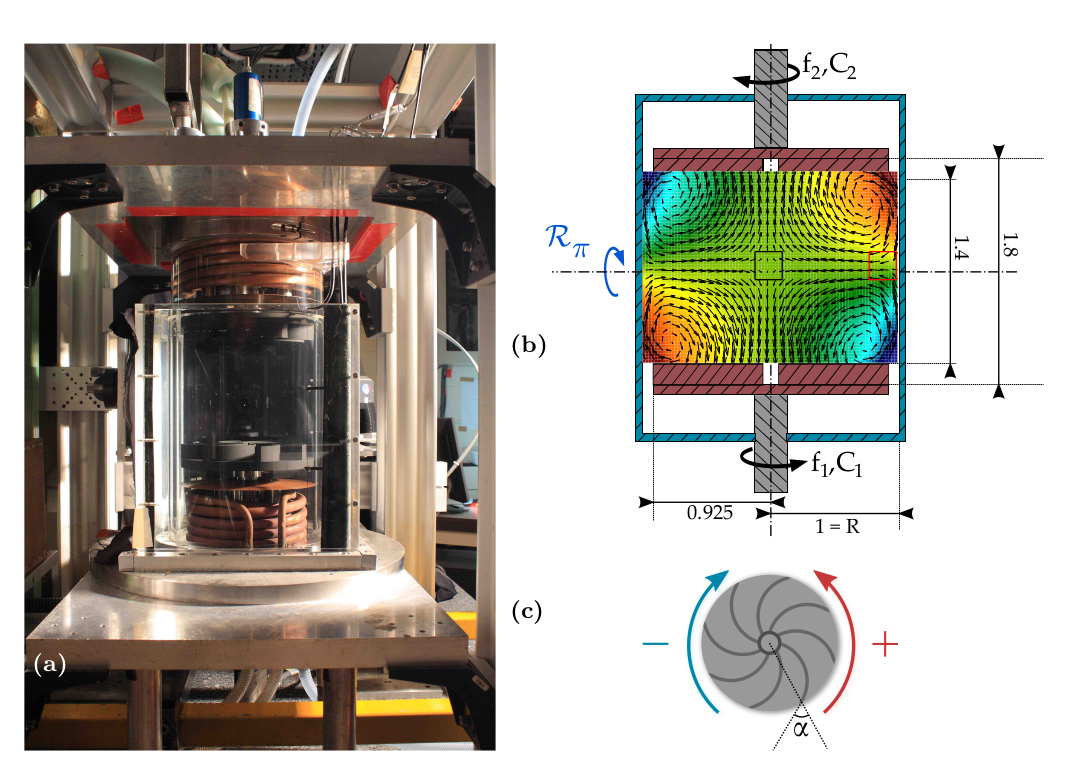
\includegraphics[width=.9\linewidth]{figs/geometrie_vk.png}
  \caption[Géométrie de von Kármán]
  {Géométrie de von Kármán. 
  (a) Photographie de la manipulation effectuée au SPEC CEA-Saclay. (b) Vue schématique du montage
  et champ de vitesse moyenné temporellement obtenu par vélocimétrie par imagerie de particules stéréoscopique.
  (c) Vue du dessus d'une des turbines (constituées d'un disque et de 8 pales courbées) 
  avec les 2 sens de rotation possibles: en bleu (-) la configuration ANTI-CONTRA 
  et en rouge (+) la configuration CONTRA.
  Figure tirée de \cite{Dubrulle-Beyond}.}
  \label{fig:geo_vk}
\end{figure}

\subsubsection{Code SFEMaNS}
\noindent SFEMaNS (\emph{Spectral/Finite Element code for Maxwell and Navier-Stokes equations})
est un code hautement parallélisé qui permet de résoudre les équations
de Navier-Stokes, les équations de Maxwell et leur couplage (magnétohydrodynamique) \cite{sfemans}.
Il se base sur une discrétisation spatiale hybride: des éléments finis 
(dans le plan méridien ($r,z$)) ainsi qu'une 
décomposition en modes de Fourier en azimut.
Toutes les simulations mentionnées dans ce rapport - la base de données traitée
par exemple - sont issues de calculs effectués avec SFEMaNS. Nous détaillons plus 
les paramètres de
simulations en sections \S \ref{sec:stat_faller} et \S \ref{sec:problematique}.\\

\noindent Le cadre de travail étant dorénavant bien défini, la problématique du 
stage en lui-même repose
sur un article que nous introduisons dans la section suivante. 

\subsection{Faller \emph{et al.}, Journal of Fluid Mechanics {\bf 914}, 2 (2021)}
\subsubsection{Données analysées}\label{sec:stat_faller}
\noindent En préambule de considérations plus dynamiques (intermittence), 
Hugues Faller effectue une analyse statistique de la turbulence de 
l'écoulement de von Kármán \cite{Faller-Intermittency}.
Il dispose d'une base de données en simulation numérique directe
ainsi que de données provenant d'expériences. Les mesures expérimentales sont issues
du carré noir central de la figure \ref{fig:geo_vk}-(b) tandis que les données
computationnelles proviennent du volume entier excluant les turbines. La discrétisation
SFEMaNS consiste en une grille de points en coordonnées cylindriques. Il y a 255 modes
de Fourier décomposant la coordonnée angulaire et donc 509 plans-$\theta$. En chaque plan,
le code associe la même triangulation en $\qty(r,z)$ générant 732 016 points. Il y a donc pour une
snapshot $\sim 3.73 \times 10^8$ points. 21 snapshots décorrélés forment l'ensemble des expériences répétées.
Les paramètres associés aux écoulements de von Kármán étudiés sont en outre listés
dans la table \ref{tab:params_vk}.
\begin{table}%[ht]
\begin{center}
\def~{\hphantom{0}}
\begin{tabular}
{|llcrrlllc|}%
%\hline \hline
 Cas &F (\SI{}{\hertz})& Points de grille &$\text{Re}\quad $ &$\epsilon (\text{adim})$ &$\eta$(\SI{}{\milli\metre})& 
$\Delta x$(\SI{}{\milli\metre})\\[3pt]
%\hline \hline
%\hline
 A &$5$&$89 \times 65$&$3.1~10^5$&$0.045$& $0.016$&$2.1$\\
%\hline
B&$5$&$77 \times 79$&$3.1~10^5$&$0.045$&$0.016$&$0.49$\\
%\hline
C&$5$&$162\times157$&$3.1~10^5$&$0.045$&$0.016$&$0.24$\\
%\hline
D&$1$&$77 \times 80$&$4.1~10^4$&$0.045$&$0.073$&$0.49$\\
%\hline
E&$1.2$&$151\times174$&$5.8~10^3$&$0.045$&$0.32$&$0.24$\\
%\hline
T-$1$ &$5$&$149\times103\times20$&$3.1~10^5$&$0.045$&$0.016$&$0.35$\\%TPIV Paul
%\hline
T-$2$ &$1$&$139\times101\times20$&$6.3~10^4$&$0.045$&$0.054$&$0.35$\\%TPIV Paul
%\hline
T-$3$ &$0.5$&$148\times103\times20$&$3.1~10^4$&$0.045$&$0.09$&$0.35$\\%TPIV Paul
%\hline
T-$4$ &$0.1$&$149\times100\times20$&$6.3~10^3$&$0.045$&$0.3$&$0.35$\\%TPIV Paul
%\hline
DNS &$\frac{1}{2\pi}$&$400\times800\times509$&$6~10^3$&$0.045$&$0.37$&$0.1$-$0.4$\\%Hugues
\end{tabular}
\caption[Paramètres décrivant les données utilisées dans l'article 
\cite{Faller-Intermittency}]{Paramètres décrivant les données utilisées dans 
l'article \cite{Faller-Intermittency}. 
$F$ est la fréquence de rotation des turbines en Hz;
$Re$ est le nombre de Reynolds basé sur $F$ et le rayon du cylindre;
$\epsilon$ est la dissipation énergétique totale adimensionnée ; $\eta$ est 
l'échelle de Kolmogorov ;
et $\Delta x$ représente la résolution spatiale dans les expériences 
(dénotées de A à T-4) et les simulations numériques directes (dénotées DNS).}
\label{tab:params_vk}
 \end{center}
\end{table}%}

Les densités de probabilité jointe entre le champ 
$\mathscr{D}^I_\ell$ et $\omega=|\git{\omega}|$ obtenues pour les données expérimentales 
et numériques sont rapportées dans les figures \ref{fig:joint_exp} et \ref{fig:joint_faller}.
Quel est le but d'observer ces quantités ? Il suffit de se rappeler de la section \S
\ref{sec:anomalous} : s'il existe un mécanisme à l'origine de la dissipation anormale,
alors il est obligatoirement relié aux singularités de la vorticité.
\begin{figure}[h]
  \centering
  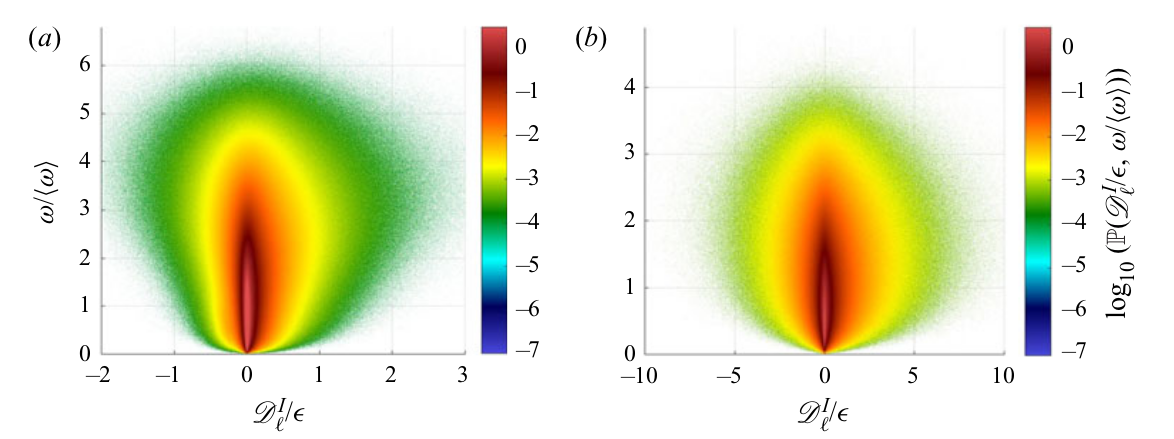
\includegraphics[width=.95\linewidth]{figs/pdf_exp.png}
  \caption[Densités de probabilité jointe pour les données expérimentales de \cite{Faller-Intermittency}]
  {Densités de probabilité jointe pour les données expérimentales.
  (a) T-4: $\ell= 3.2\eta$ (3 $\times 10^4$ snapshots). (b) T-2: 
  $\ell = 17.9\eta$ (1.02 $\times 10^4$ snapshots). Figure tirée de \cite{Faller-Intermittency}.}
  \label{fig:joint_exp}
\end{figure}
\begin{figure}[h]
  \centering
  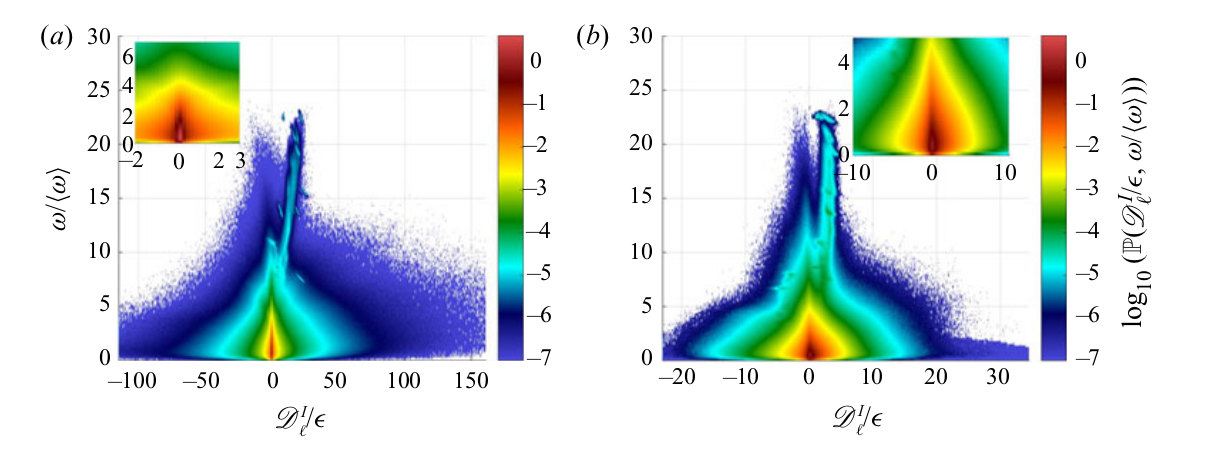
\includegraphics[width=.95\linewidth]{figs/pdf_dns.png}
  \caption[Densités de probabilité jointe pour les données simulées de \cite{Faller-Intermittency}]
  {Densités de probabilité jointe pour les données simulées.
  (a) $\ell= 1.06\eta$. (b) $\ell = 26.5\eta$. Figure tirée de \cite{Faller-Intermittency}.} 
  \label{fig:joint_faller}
\end{figure}
Faller obtient notamment un étrange jet de corrélations dans la gamme de densité 
de probabilité autour de $10^{-5}$ (voir la figure \ref{fig:joint_faller}) qui est restée inexpliquée à ce jour.
\emph{Dans tout ce rapport, nous ferons spécifiquement r\'ef\'erence \`a ce jet par l'appelation 
{\bf oreille de lapin}}.

\subsubsection{Corrections et nouvelles simulations}\label{sec:problematique}
\noindent On arrive à un des questionnements majeurs de mon stage; à savoir 
{\bf quelle est l'origine de l'oreille de lapin ?} Mes superviseurs ont établi
une liste d'erreurs dans les calculs SFEMaNS de Faller qui mettent en doute 
la validité des résultats obtenus:
\begin{itemize}
  \item $\grad\cdot \git{u}$ n'est pas tout à fait égal à 0;
  \item le filtrage est mauvais sur l'axe du cylindre;
  \item les conditions aux limites sont questionnables ;
  \item $\mathscr{D}^I$ comportant un terme de divergence, son intégration apporte
        des effets indésirables. En effet, les conditions aux limites peuvent créer des quasi-
        irrégularités et $\mathscr{D}^I$ peut les capturer par le théorème de la divergence.
        Or on s'intéresse \ul{exclusivement} aux transferts inter-échelle ici, 
        c'est-à-dire aux transferts qui ne dépendent pas des conditions aux limites.
\end{itemize}
Sur la base de ces pistes, nous disposons d'une nouvelle base de données corrigées
avec rigoureusement les mêmes paramètres que ceux de Faller.
Nous pouvons finalement introduire dans la suite l'analyse statistique des données
en question - sujet qui est au coeur de mon stage. 

\section{Module d'analyse statistique}
\noindent L'objectif du stage étant d'étudier la statistique de l'écoulement de von Kármán turbulent,
mon travail a consisté à développer un code dédié à cette analyse en utilisant le langage Python. 

\subsection{Code \texttt{von-Karman-PostProcess}}\label{sec:code-VK}
\noindent Nous avons programmé un module d'analyse statistique permettant de calculer toutes
les grandeurs mentionnées dans la section \S\ref{sec:outil_turb}:
\href{https://gitlab.lisn.upsaclay.fr/allaglo/von-karman-postprocess}
{von-Karman-PostProcess}. En particulier, nous avons cherché à optimiser les performances
du dit module en implémentant une version accélérée sous la branche \texttt{gpus}
du projet (voir section \S \ref{sec:gpus} pour des explications sur l'utilisation de 
GPUs sur Python). Des exemples d'utilisation sont rapportés
dans un \href{https://gitlab.lisn.upsaclay.fr/allaglo/von-karman-postprocess/-/blob/main/tutorial/tutorial.ipynb}{tutoriel}
partagé dans le projet. Cette section décrit les mathématiques sous-jacentes à
toutes ces fonctions. On considère dans toute la suite un champ \emph{scalaire} et 
\emph{continu} quelconque $A$ défini sur un volume $\Omega$ décrit temporellement pendant une durée $T$.
La base de données (classe \texttt{Database}) fournit la structure de données
d'ordre 3 suivante:
$\qop{A}_{\git{r},p}^t$ avec $\git{r}$ qui indice un point de la grille, $p$ le plan
et $t$ le temps.

\subsubsection{Valeurs moyennes}
\noindent On définit le moment {\bf spatial} de $A$ à l'ordre $n\neq 1$ comme
\begin{align}
    \mean{A^n}_{\Omega}(t) = \dfrac{1}{\text{Vol}~\Omega}\mathlarger{\mathlarger{\int_\Omega}}
                 \qty(A(\g{r},t)-\mean{A}_{\Omega}(t))^n\dd^3\g{r},
    \label{eq:moment_n_space}
\end{align}
avec $\displaystyle\text{Vol}~\Omega = \int_\Omega \dd^3\git{r}$. Bien évidemment,
il faut discrétiser l'équation~\eqref{eq:moment_n_space}.
La mesure d'intégration $\dd^3\g{r}$ est stockée dans un tableau $\qop{w}_{\git{r}}$.
On va expliciter le calcul de la moyenne qu'on généralisera ensuite
pour un moment quelconque. Nous obtenons :
\begin{align}
    \mean{A}_{\Omega}(t) = \dfrac{\mathlarger{\mathlarger{\sum_{p\in\qop{P}}\sum_{\git{r}\in\text{mesh}}}}
               \qop{A}_{\git{r},p}^t\qop{w}_{\git{r}}}
               {\mathlarger{\mathlarger{\sum_{p\in\qop{P}}\sum_{\git{r}\in\text{mesh}}}}
               \qop{w}_{\git{r}}},
    \label{eq:moy_disc}
\end{align}
qui se généralise à l'ordre $n$ en 
\begin{align}
    \mean{A^n}_{\Omega}(t) = \dfrac{\mathlarger{\mathlarger{\sum_{p\in\qop{P}}\sum_{\git{r}\in\text{mesh}}}}
               \qty(\qop{A}_{\git{r},p}^t-\mean{A}_\Omega(t))^n\qop{w}_{\git{r}}}
               {\mathlarger{\mathlarger{\sum_{p\in\qop{P}}\sum_{\git{r}\in\text{mesh}}}}
               \qop{w}_{\git{r}}}.
\end{align}
Seule l'opération~\eqref{eq:moy_disc} est déjà implémentée sous \texttt{numpy.average}.
Il suffit donc d'appliquer~\eqref{eq:moy_disc} sur le champ $\qty(\qop{A}_{\git{r},p}^t-\mean{A})^n$
pour obtenir le moment à l'ordre $n$. \\

\noindent Les statistiques {\bf temporelles} s'encodent selon le même principe.
Les statistiques sont ici définies selon:
\begin{align}
    \mean{A^n}_{T}(\g{r}) = \mathlarger{\dfrac{1}{T}}\mathlarger{\mathlarger{\int_T}}
                 \qty(A(\g{r},t)-\mean{A}_{T}(\g{r}))^n\dd t,
\end{align}
La discrétisation est immédiate après ce qui précède:
\begin{align}
    \mean{A^n}_{T}(\git{r},p) = \mathlarger{\dfrac{1}{N_{\qop{T}}}}\mathlarger{\mathlarger{\sum_{t\in\qop{T}}}}
               \qty(\qop{A}_{\git{r},p}^t-\mean{A}_T(\git{r},p))^n
\end{align}
On notera bien que, dans un cas, on obtient un tenseur d'ordre 1 et, dans l'autre, un tenseur
d'ordre 2. 

\subsubsection{Lois de probabilité}
\noindent Afin de calculer la fonction de densité de $A$, il faut encore procéder à
l'usage d'estimateurs. Il s'agit ici essentiellement de "compter" combien de fois
les données égalisent une certaine valeur $a$. Dans le cas continu,
on considère plutôt un intervalle centré sur $a$ et de largeur choisie $\delta a$. Il y a une
légère subtilité: $A$ étant accessible non pas localement mais autour d'un élément
de volume, une mesure (un compte) doit par conséquent être pondéré par le jacobien associé.
Formellement, l'estimateur $f^*$ de la fonction de densité de $A$ est enfin:
\begin{align}
    f^*(a) = \dfrac{1}{N\delta a}\mathlarger{\sum_{t\in\qop{T}}\sum_{p\in\qop{P}}
    \sum_{\git{r}\in\text{mesh}}}H\qty(\dfrac{\delta a}{2}-
    \big\vert\qop{A}_{\git{r},p}^t-a\big\vert)\qop{w}_{\git{r}},
    \label{eq:estim_pdf}
\end{align}
avec $\qty(H(x) = 1~\text{si}~x\geq 0~\text{et}~0~\text{sinon})$ et $N$ le nombre
de mesures TOTALES. Pour que $f^*$ soit bien une densité de {\bf probabilité}, il faut
que les poids soient \underline{normalisés} au sens $
\qop{w}_{\git{r}}\leftarrow\displaystyle\dfrac{\qop{w}_{\git{r}}}{
    \displaystyle\sum_{t\in\qop{T}}\sum_{p\in\qop{P}}\sum_{\git{r}\in\text{mesh}}\qop{w}_{\git{r}}}$.
L'opération~\eqref{eq:estim_pdf} est implémentée sous \texttt{numpy.histogram}.\\
Le principe est semblable lorsque l'on considère 2 champs $A$ et $B$:
\begin{align}
    f^*(a,b) = \dfrac{1}{N\delta a\delta b}\mathlarger{\sum_{t\in\qop{T}}\sum_{p\in\qop{P}}
    \sum_{\git{r}\in\text{mesh}}}H\qty(\dfrac{\delta a}{2}-
    \big\vert\qop{A}_{\git{r},p}^t-a\big\vert)
    H\qty(\dfrac{\delta b}{2}-
    \big\vert\qop{B}_{\git{r},p}^t-b\big\vert)\qop{w}_{\git{r}}^2.
    \label{eq:joint_pdf}
\end{align}
Il faut néanmoins utiliser dans ce cas \texttt{histogram2d}. En anticipation de la
prochaine section, on notera bien qu'en aucune façon on devrait avoir 
$f^*(a,b) \neq f^*(a)f^*(b)$. En effet, 
même s'il est vrai que l'on échantillonne bi-dimensionnellement les grandeurs 
\underline{pour calculer les pdfs} ({\it{probability density function}}), c'est plutôt les échantillons de 
{\bf l'espace des expériences aléatoires} qui importent~! L'expression~\eqref{eq:joint_pdf}
parcourt bien le dit espace une seule fois et non deux fois.\\

\noindent On appelle $f_\alpha$ la densité de probabilité \emph{marginale} d'un champ
$\alpha$. La densité de probabilité jointe de deux évènements A et B quant à elle sera notée $f_{A,B}$. 
L'intuition probabilistique permet de quantifier la probabilité d'un événement
$A$ \emph{étant donnée} la réalisation d'un événement $B$ comme:
\begin{align}
    \mathbb{P}\qty(B|A) = \dfrac{\mathbb{P}\qty(A\cap B)}{\mathbb{P}(A)}.
\end{align}
Pour des variables à densité, l'idée est évidemment généralisable:
\begin{align}
    f_{B|A}(a,b) = \dfrac{f_{A,B}(a,b)}{f_{A}(a)}.
    \label{eq:loi_cond}
\end{align}
Pour échantillonner cette loi, il suffit d'obtenir $f_{A,B}(a,b)$. 
En effet, $f_{A}(a)$ étant une loi marginale, on peut se passer
d'effectivement calculer la pdf simple. 
Échantillonner~\eqref{eq:loi_cond} revient donc à une simple division de tableaux
élément par élément. L'espérance conditionnelle découle enfin:
\begin{align}
    \mathbb{E}\qty(B|A) &= \int_{\Omega_B}b\cdot f_{B|A}(a,b)\dd b~\text{(variable continue)};\\
    \mathbb{E}\qty(B|A) &= \sum_b~b\cdot\dfrac{f_{A,B}(a,b)}{f_{A}(a)}\delta b~\text{(variable échantilonnée)}.
\end{align}
On a donc vu qu'en général $f_{A,B} = f_{A}\cdot f_{B|A}$ avec $f_{B|A}$ la probabilité 
que B se réalise sachant que A s'est réalisé. $A$ et $B$ sont {\bf indépendants} 
si $f_{A,B} = f_A\cdot f_B$. Cela revient à dire que trouver $b$ n'influe pas
sur le fait de trouver $a$: il n'existe donc bien aucune corrélation entre $A$ et $B$. \\
Le coefficient de corrélation de $A$ et $B$ n'est pas vraiment
pertinent pour nous car il ne quantifie pas {\bf localement} les corrélations.
Il est plus pertinent de considérer la corrélation :
\begin{align}
    \mathcal{C}(A,B) = \dfrac{f_{A,B}}{f_{A}f_{B}}
    \label{eq:correlations}
\end{align}
qui mesure localement si la loi de Bayes ($f_{A,B}=f_{A}f_{B}$) s'applique ou pas. 
Cette corrélation $\mathcal{C}(A,B)$ varie entre 0 (si le numérateur vaut zéro) et 
l'infini. Elle vaut 1 quand les évènements sont indépendants,  $\mathcal{C}(A,B)< 1$ 
quand les variables sont anti-corrélées et  $\mathcal{C}(A,B)> 1$ quand les variables sont corrélées.\\

\noindent Pour calculer~\eqref{eq:correlations}, on pourrait croire qu'il suffit
d'appeler la fonction \texttt{histogram2d} et \texttt{histogram} de \texttt{numpy} et procéder
à une division élément par élément mais ce n'est pas la méthode la plus
efficace. Avec la seule fonction de probabilité jointe, on peut obtenir
toutes les grandeurs. Les densités marginales peuvent en effet être obtenues
à partir de la probabilité jointe: la probabilité d'avoir juste $A$
égalise la probabilité d'avoir $A$ et $B$ {\bf quel que soit $B$}. Mathématiquement,
\begin{align}
      f_A(a) &= \int_{\Omega_B}f_{A,B}(a,b)\dd b~\text{variable continue} \\
      f_A(a) &= \sum_b f_{A,B}(a,b)\delta b~\text{variable échantillonnée}.
\end{align}
La corrélation locale peut donc être obtenue à partir de la seule probabilité jointe. 

\subsubsection{Localisation des statistiques}
\noindent En plus des statistiques d'ensemble, on peut comparer les statistiques 
entre sous-espaces du volume de l'écoulement. En l'occurence, en prévision des résultats
rapportés en section \S\ref{sec:results}, on considère trois sous-espaces pertinents:
\begin{itemize}
      \item {\bf \emph{bulk}}: $|z|\leq 0.1,r\leq 0.1$ - pertinent pour la comparaison
            avec les résultats des expériences
      \item {\bf \emph{interior}}: $|z|\leq 0.69$ - pour considérer l'écoulement en dehors
            des pales
      \item {\bf \emph{penal}}: \noindent parce que le champ de vitesse associé 
      au fluide n'existe pas dans la région des turbines (qui sont solides),
      le code SFEMaNS fournit un champ \texttt{penal}$=\qop{I}_{\git{r},p}^t$ indiquant le poids effectif des
      points échantillonnés (par-delà le jacobien). En voyant un peu trop ce champ comme
      une indicatrice, on pourrait croire qu'il suffit de multiplier tous les champs
      d'intérêt par ce dernier. \underline{C'est faux}: il faut plutôt pondérer le poids
      statistique par ce dernier afin d'effectivement comptabiliser ou non un point. Dans
      le cas contraire, on modifie la valeur du champ en lui-même, ce qui perturbe inévitablement
      les statistiques. \\
      Pour toute fonction retournant des statistiques \texttt{func}$\qty(\qop{w}_{\git{r}})$ 
      dépendant de la base de données à travers le poids statistique, la pénalisation
      implique la transformation globale du code:
      \begin{align}
          \texttt{func}\qty(\qop{w}_{\git{r}}) \rightarrow \texttt{func}\qty(\qop{I}_{\git{r},p}^t
                                              \qop{w}_{\git{r}}).
      \end{align}
      On notera qu'on peut désormais définir un nouveau poids statistique $\tilde{\qop{w}}_{\git{r},p}^t
      = \qop{I}_{\git{r},p}^t\qop{w}_{\git{r}}$ qui est un tenseur d'ordre 3 selon
      la structure actuelle de la base de données. On considère qu'un point
      appartient bien à l'écoulement si $\texttt{penal}>0.8$ et, dans ce cas, on fixe la valeur de penal
      à 1. Dans le cas contraire, la valeur est imposée à 0.
\end{itemize}

\subsection{Gestion de la mémoire}

\noindent Ce stage fut une occasion pour moi d'entrouvrir une porte sur le monde du 
\emph{High Performance Computing} (HPC) : bases de données massives, clusters, 
supercalculateurs, programmation dirigée GPUs, etc. Le traitement de données 
massives peut s'avérer en outre une étape cruciale dans le déroulé d'un projet 
de recherche en physique. Une partie importante de mon travail a ainsi été de 
pouvoir appliquer les statistiques développées dans 
la section \S \ref{sec:code-VK} sur une grande base de données. Cette section 
technique explique comment j'ai dû restructurer 
la base de données à cet effet. Elle peut être ignorée en première lecture si 
le lecteur s'intéresse
aux résultats physiques décrits dans la section \S \ref{sec:results}.

\subsubsection{Restructuration des données}
\noindent La base de données fournit des champs très gourmands en termes de ressources:
pour un champ 1D, il faut compter 77 GB et donc le triple pour trois dimensions.
Construire un workload sur deux champs entiers est possible mais nécessite
au minimum 150 GB de RAM pour deux champs 1D et 300 GB pour un champ 1D et un champ 3D.
Réserver 300 GB de RAM est possible sur Lab-IA, la machine dont on dispose : 
il y a 2 noeuds sur 12 offrant 
cette possibilité (qui ont 384 GB de mémoire). Le temps d'attente sera cependant 
plus long qu'à l'accoutumée puisqu'il
faudra réserver un noeud quasiment entier.\\
La structure des données étant nativement ordonnée et de surcroît d'ordre 3 
($\qop{A}_{\git{r},p}^t$ avec $\git{r}$ indiquant la grille, $p$ le plan et $t$ le champ instantané), 
un moyen rapide de remédier au problème est de restructurer les données.\\

\noindent Le moyen le plus trivial et en même temps le plus intelligent est de découper
chaque champ temporellement: on génère alors 28 paquets ordonnés de taille variant
entre 2.33 GB et 8.33 GB. Par-delà l'évidente optimisation en ce qui concerne la
gestion de la mémoire, on peut dorénavant comparer les statistiques entre ensembles décorrélés. 
Si l'on générait plutôt les paquets aléatoirement (par exemple en mélangeant temps et espace), 
aucun résultat intermédiaire ne serait
exploitable puisque seule la recombinaison ultime des paquets fournirait le résultat
initialement recherché.

\subsubsection{Lectures en parallèle}
\noindent La base de données étant \emph{délayée}, les données
sont effectivement importées sur la RAM uniquement si on donne cette instruction.
Cette façon de procéder permet de charger en mémoire \ul{uniquement} ce qui nous sert, chose
qui est très commode pour une restructuration des données.
À ce propos, le module \texttt{Dask} permet d'effectuer des opérations en parallèle
sur des objets délayés. Selon les dimensions des données, on peut alors optimiser
le chargement de ces données en choisissant un nombre de coeurs adéquat. En pratique, 
il s'agit de faire en sorte que chaque thread puisse s'occuper indépendamment
d'une partie ni trop grosse ni trop petite des données totales (il est important 
que le nombre de "chunks" ainsi
formés soit entier). 
Le chargement des données est enfin optimisé en chargeant 14 chunks indépendamment
à l'aide des instructions suivantes :
\vspace{.2cm}

\noindent\begin{pythoncode}{label=lst:rechunk,colback=Red!5!white,colframe=Red,coltitle=black}
  {Chunking des données délayées sur 14 threads}
  from vkcupp import Stats
  import dask.array as da

  db_path = '...'
  pp = Stats(db_path, 'penal')         # getting the PostProcessing module
  data = pp.db                         # database dictionnary
  P, N = pp.dims[2], pp.dims[3]        # p,r dimensions in data struct

  field = data[key]['field']           # field is delayed at this point
  field = field.rechunk((1,1,P,N//14)) # field is chunked into 14 blocks
  field = field.compute()              # parallelized-loading on the RAM
\end{pythoncode}

\subsubsection{Tâches de travail (workloads) de type probabilité jointe}\label{sec:workloads}
\noindent Des détails techniques de la mise en place des workloads sont donnés
en secion \S \ref{sec:tech_workloads}. 
L'idée étant à terme de recombiner les histogrammes, il est très important
que les intervalles échantillonnés sur chaque workload soient identiques. La méthode
\texttt{Stats.joint\_pdf} que j'ai codée détermine nativement les intervalles automatiquement;
cela demeure problématique puisque les intervalles varient entre chaque ensemble.
Pour calculer des probabilités jointes, il faut alors en premier lieu calculer
les intervalles des champs \ul{totaux} et les fournir à chaque workload. On comprend
vite que le problème de la mémoire demeure pour ce calcul: la solution
est naturellement de procéder à cette même restructuration de données. Concrètement,
il s'agit de lançer un job récupérant l'étendue (range) de chaque workload.
L'ensemble des workloads partitionnant les données totales, en concaténant les intervalles
ainsi obtenus, l'étendue (range) globale est simplement constituée du min et du max de l'ensemble
$\left\{\left\{\qop{A}_{\text{min}}^t,\qop{A}_{\text{max}}^t\right\}_t\right\}$ aplati. \\

\noindent Nous donnons dans le script \ref{lst:gpu_work} un script permettant
de calculer la densité de probabilité jointe entre les champs $\mathscr{D}^{I}_{\ell=1.06\eta}$ et $\omega$
avec champ de pénalisation à l'aide d'un GPU.

\vspace{.2cm}

\noindent\begin{pythoncode}{label=lst:gpu_work,colback=Red!5!white,colframe=Red,coltitle=black}
  {Workloads séquentiels sous GPUs}
  import os
  from vkcupp import Stats
  import cupy as cp
  import dask.array as da

  db_path = '...'
  pp = Stats(db_path, 'penal')           # getting the PostProcessing module
  data = pp.db                           # database dictionnary
  P, N = pp.dims[2], pp.dims[3]          # p,r dimensions in data struct

  # Defining the rechunked+delayed fields
  DI_delayed = data['D002_DR']['field'].rechunk((1,1,P,N//14))          
  w_delayed = data['omega']['field'].rechunk((3,1,P,N//14)) 

  # Run params
  bags = 28
  bins = 2000
  w_min, w_max = 0, 402.535165           # computed externally
  DI_min, DI_max = -1.893386, 3.594616   # computed externally
  ranges = [[DI_min, DI_max], [w_min, w_max]]
  os.mkdir('slices')                     # for saving purposes
  s = slice(None)

  # Sequential workloads
  for t in range(bags):
    print('###############################################################')
    print('Frame %d' %t)
    
    # Loading the sliced fields
    pp.set_penal(s, [t], s, s)           # automatically sent to CUDA
    DI, w = [x[:, [t], :, :].compute() for x in [DI_delayed, w_delayed]]
    print('Loaded all fields')

    # Transferring to CUDA
    DI, w = [cp.array(x, copy=False) for x in [DI, w]]
    print('Transferred all fields to CUDA')

    # CUDA calculations
    w = pp.norm(w)                       
    print('Computed w norm')

    DI_w, edges = pp.joint_pdf(DI, w_norm, bins, ranges, log=False, \
                               save='slices/iter_%d' % (t))
    
    print('Computed joint_pdf')
\end{pythoncode}

\noindent Le script \ref{lst:gpu_work} sauvegarde alors les densités de probabilité
jointes dans des fichiers binaires; la suite des opérations est naturellement de
correctement recombiner les résultats. Les slices temporelles partionnant l'espace
des expériences aléatoires, la procédure correcte est de sommer toutes les réalisations
bin par bin. Quid de la normalisation ? Si les pdfs sommées sont déjà normalisées,
alors on vérifie pour chaque histogramme $\qop{H}^t$ (les éléments de surface sont identiques
pour tous puisqu'on a imposé une étendue (range) commune):
\begin{align}
    &\sum_{i,j}\qop{H}^t_{i,j}\qop{W}_{i,j} = 1 \\
    \Rightarrow~&\sum_{t}\sum_{i,j}\qop{H}^t_{i,j}\qop{W}_{i,j} = N_{\text{bags}} \\
    \Rightarrow~&\sum_{i,j}\tilde{\qop{H}}_{i,j}\qop{W}_{i,j} = 1,~\text{avec}~
    \tilde{\qop{H}}_{i,j} = \dfrac{1}{N_\text{bags}}\sum_t\qop{H}^t_{i,j}.
\end{align}
Le script \ref{lst:recomb} permet enfin d'obtenir les histogrammes complets.

\vspace{.2cm}

\noindent\begin{pythoncode}{label=lst:recomb,colback=Red!5!white,colframe=Red,coltitle=black}
  {Recombinaison des probabilités jointes}
  from vkcupp import Stats
  import numpy as np
  
  db_path = '...'
  pp = Stats(db_path, 'penal')           # getting the PostProcessing module
  bins = 2000
  bags = 28

  # Gathering all partial joint pdfs
  joints = []
  for t in range(bags):
    hist = np.fromfile('slices/iter_%d' % (t))
    DI_w = pp.load_reshaped(hist, bins)
    joints.append(DI_w)

  # Full hist
  DI_w_full = (np.sum(np.array(joints), axis=0)/bags)
\end{pythoncode}

\section{Résultats et discussion}\label{sec:results}
Nous décrivons dans cette section les résultats obtenus avec le module de traitement 
statistique appliqué sur la base de données restructurée. Nous allons comparer nos 
résultats à ceux publiés par l'équipe~\cite{Faller-Intermittency}.

\subsection{Comparaison avec Faller \emph{et al.}~\cite{Faller-Intermittency}}
Nous comparons d'abord avec les résultats issus des simulations numériques directes 
(Direct Numerical Simulations, DNS), puis avec les résultats issus de l'expérience
 von Kármán située au laboratoire SPEC (CEA, Saclay) sous la direction de Bérengère Dubrulle.
\subsubsection{Comparaison avec les résultats de DNS} % DR-w, penal, l=1,2
\begin{figure}[H]
  \centering
  \begin{subfigure}[b]{0.48\linewidth}
  \centering
  \includegraphics[width=\textwidth]{figs/figs_rapport/joint_D001_DR_omega_penal.jpg}
  \caption{Probabilité jointe de $\frac{\mathscr{D}^I_{\ell=1.06\eta}}{\epsilon}$ et 
  $\frac{\omega}{\mean{\omega}}$}
  \end{subfigure}
  \begin{subfigure}[b]{0.48\linewidth}
    \centering
    \includegraphics[width=\textwidth]{figs/figs_rapport/joint_D002_DR_omega_penal.jpg}
    \caption{Probabilité jointe de $\frac{\mathscr{D}^I_{\ell=26.5\eta}}{\epsilon}$ et 
    $\frac{\omega}{\mean{\omega}}$}
    \end{subfigure}
  \caption{Statistiques de $\mathscr{D}^I$ et $\omega$ aux échelles $\ell=1.06\eta$ et 
  $\ell=26.5\eta$
           avec pénalisation des turbines}
  \label{fig:DR_penal}
\end{figure}
\noindent La figure \ref{fig:DR_penal} rapporte les densités de probabilité jointe 
pour les champs $\mathscr{D}^I$ et $\omega$ pour deux échelles de filtrage distinctes. 
Près de l'échelle de Kolmogorov (fig. \ref{fig:DR_penal}-a), la première observation 
à faire est la différence majeure d'étendue de 
$\frac{\mathscr{D}^I_{\ell=1.06\eta}}{\epsilon}$ avec les résultats de Faller 
(cf. figure \ref{fig:joint_faller}). Dans notre cas, les évènements hors de 
l'intervalle $\qty[-15,20]$ (normalisé par $\epsilon$) sont quasiment improbables. 
Faller parvient à capturer l'étendue $\qty[-100,150]$. 
Cette différence n'est pas présente pour la grande échelle de filtrage 
(fig. \ref{fig:DR_penal}-b) où nos étendues demeurent à peu près similaires 
même si nous ne parvenons que difficilement à reproduire des probabilités 
inférieures à $10^{-5}$. La difficulté à aller chercher des probabilité très 
faibles peut s'expliquer par un argument numérique: la taille des \emph{bins}. 
Les graphiques de Faller donnent l'impression d'être beaucoup moins résolus que 
les nôtres (10000$\times$10000). Des bins trop étroits ont l'avantage de la 
résolution mais peuvent malgré tout manquer à rendre compte de \emph{tendances}. 
Autrement dit, pour des évènements effectivement plus rares, il vaut mieux avoir 
une plus grosse réserve permettant au moins de capturer un certain nombre de 
réalisations. En capturant seulement un bin infinitésimal, on ne peut presque rien visualiser. \\
En ce qui concerne l'étroitesse de l'abscisse de la probabilité jointe de la 
figure \ref{fig:DR_penal}-a, le fait qu'elle apparaisse seulement à très faible
 échelle suggère que c'est un problème lié au filtrage sur l'axe, seule source 
 
 de différence liée à $\ell$. \\
Cependant, les zooms présentés en insert dans la figure \ref{fig:DR_penal} 
présentent une certaine similarité avec les résultats de \cite{Faller-Intermittency} 
(au moins pour la grande échelle). \\

\noindent Le point essentiel à désormais relever est {\bf l'absence totale d'oreille 
de lapin}. Il existe certains structures ressemblant à des "blobs" mais qui 
n'apparaissent pas quand nous calculons les probabilités jointes dans les autres 
sous-espaces (\texttt{bulk} et \texttt{interior}). Nous pouvons en déduire que 
ces blobs sont des artefacts liés à l'écoulement \ul{entre} les pales des turbines. 
L'origine de l'oreille de lapin est à notre niveau d'analyse multi-factorielle: 
la divergence non-nulle ainsi que les mauvaises conditions aux bords ont pu toutes 
les deux participer à cette structure corrélée. 

\noindent Pour conclure cette comparaison entre résultats numériques, nous 
retiendrons surtout que les bonnes statistiques s'étalent moins à basse échelle 
et sont donc plus localisées. Les transferts vers les échelles de plus en plus 
basses sont plus regroupés vers des valeurs plus faibles des transferts inter-échelle.

\subsubsection{Comparaison avec les résultats expérimentaux}\label{sec:res_exp} % DR-w, bulk, l=1,2
\begin{figure}[H]
  \centering
  \begin{subfigure}[b]{0.48\linewidth}
  \centering
  \includegraphics[width=\textwidth]{figs/figs_rapport/DDR1_omega_bulk.jpg}
  \caption{Probabilité jointe de $\frac{\mathscr{D}^I_{\ell=1.06\eta}}{\epsilon}$ 
  et $\frac{\omega}{\mean{\omega}}$}
  \end{subfigure}
  \begin{subfigure}[b]{0.48\linewidth}
    \centering
    \includegraphics[width=\textwidth]{figs/figs_rapport/DDR2_omega_bulk.jpg}
    \caption{Probabilité jointe de $\frac{\mathscr{D}^I_{\ell=26.5\eta}}{\epsilon}$ 
    et $\frac{\omega}{\mean{\omega}}$}
    \end{subfigure}
  \caption{Statistiques de $\mathscr{D}^I$ et $\omega$ aux échelles $\ell=1.06\eta$ 
  et $\ell=26.5\eta$
           dans la région bulk}
  \label{fig:DR_bulk}
\end{figure}
\noindent La figure \ref{fig:DR_bulk} représente les mêmes quantités que la figure 
\ref{fig:DR_penal} sauf qu'on considère désormais la région \texttt{bulk} uniquement 
(on reproduit les mesures des expérimentateurs en quelque sorte). Même si les données 
expérimentales formant la figure \ref{fig:joint_exp} ont des échelles de Kolmogorov 
ainsi que des échelles de filtrage différentes, nous pouvons au moins mentionner 
quelques idées intéressantes émergeant de la comparaison. Même si nous parvenons à 
accéder à des intervalles de probabilité similaire, nos structures préservent un 
caractère dissymétrique contrairement aux statistiques des expérimentateurs. Au 
centre du cylindre, on s'attendrait plutôt à une turbulence statistiquement 
quasi-homogène et quasi-isotrope car la zone de mesure est loin des turbines 
(qui entrainent le fluide) et des parois (qui imposent les conditions aux limites). 
Cela semble dire que la dissymétrie perdure même pour une turbulence homogène et 
isotrope. Ce point nécessite de plus amples investigations.\\

Dans cette section, nous avons cherché à identifier les différentes causes d'écart 
(cf. section \S \ref{sec:problematique}) entre les résultats de \cite{Faller-Intermittency} 
et nos résultats. Il nous semble que le problème à l'axe a bien été identifié, les 
soucis liés aux conditions aux limites et à la non-divergence du champ de vitesse 
restent plus insaisissables. Nous nous intéressons maintenant plus en détail à la 
distinction entre l'ancienne et la nouvelle dissipation anormale dérivée analytiquement.

\subsection{Comparaison entre $\mathscr{D}^u_\ell$ et $\mathscr{D}^I_\ell$}
Comme souligné dans la section \S \ref{sec:anomalous}, ces deux quantités diffèrent 
d'un terme en gradient. Nous allons mesurer l'impact de cette différence.
\subsubsection{Probabilités jointes} % renormaliser les graphs + corrélations
\begin{figure}[H]
  \centering
  \begin{subfigure}[b]{0.48\linewidth}
  \centering
  \includegraphics[width=\textwidth]{figs/figs_rapport/joint_D001_DR_Du_l1.jpg}
  \caption{Probabilité jointe de $\mathscr{D}^I_{\ell=1.06\eta}$ et 
  $\mathscr{D}^u_{\ell=1.06\eta}$}
  \end{subfigure}
  \begin{subfigure}[b]{0.48\linewidth}
    \centering
    \includegraphics[width=\textwidth]{figs/figs_rapport/joint_D002_DR_Du_2.jpg}
    \caption{Probabilité jointe de $\mathscr{D}^I_{\ell=26.5\eta}$ et 
    $\mathscr{D}^u_{\ell=26.5\eta}$}
    \end{subfigure}
  \caption{Évènements simultanés entre $\mathscr{D}^I (=\mathscr{D}^{DR})$ et $\mathscr{D}^u$}
  \label{fig:dudr_joint}
\end{figure}
\noindent Nous pouvons commencer par comparer les deux champs du point de vue de 
leur probabilité conjointe de réalisation. La figure \ref{fig:dudr_joint} rend 
compte de leur densité jointe pour les deux échelles déjà rencontrées précédemment. 
On remarque, très grossièrement, un contour ovoïde incliné sur la droite $y=x$ pour 
ces deux échelles. La déformation en $y=x$ suggère bien que les deux termes disposent 
d'une nature très similaire.
%
À basse échelle, on retrouve un véritable "oeuf" ; à grande échelle, on observe une 
déformation type "aile de papillon" comportant des lignes de dilatation quasiment 
dans toutes les directions.  
Cependant, on remarque que, pour $\ell\approx\eta$, il existe une ligne de 
dilatation pour $\mathscr{D}^u$ autour de 0. On comprend alors que $\mathscr{D}^I$ 
capture plus d'évènements qu'il n'en devrait: le terme en divergence contribue 
davantage que les simples transferts.


%Elles se raréfient à basse échelle. Cela stipule bien que, plus l'échelle est petite, 
%plus on a du mal à capturer les transferts inter-échelle (le terme supplémentaire en 
%divergence brouille le tout). 

\subsubsection{Corrélations}
\begin{figure}[H]
  \centering
  \begin{subfigure}[b]{0.48\linewidth}
  \centering
  \includegraphics[width=\textwidth]{figs/figs_rapport/corr_D001_DR_Du_l1.jpg}
  \caption{Corrélations entre $\mathscr{D}^I_{\ell=1.06\eta}$ et $\mathscr{D}^u_{\ell=1.06\eta}$}
  \end{subfigure}
  \begin{subfigure}[b]{0.48\linewidth}
    \centering
    \includegraphics[width=\textwidth]{figs/figs_rapport/corr_D002_DR_Du_2.jpg}
    \caption{Corrélations entre $\mathscr{D}^I_{\ell=26.5\eta}$ et $\mathscr{D}^u_{\ell=26.5\eta}$}
    \end{subfigure}
  \caption{Corrélations entre $\mathscr{D}^I (=\mathscr{D}^{DR})$ et $\mathscr{D}^u$}
  \label{fig:dudr_correl}
\end{figure}
\noindent La figure \ref{fig:dudr_correl} complète la figure \ref{fig:dudr_joint} 
en considérant les corrélations définies par l'équation~\eqref{eq:correlations}. 
L'avantage est criant: on n'a plus besoin de "deviner" les motifs (patterns) 
derrière la probabilité, ils apparaissent d'eux-mêmes. Ainsi, on voit directement 
que les lignes de dilatation (les traces bleues dans les graphes) sont anti-corrélées 
(car $C(A,B) < 1$) et d'autant plus brouillées que l'échelle du filtrage est grande. 
Que signifie l'anti-corrélation ? Il y a anti-corrélation en $(a,b)$ lorsque la 
probabilité que $A$ vaille $a$ devient d'autant plus faible lorsque la probabilité 
que $B$ vaille $b$ augmente (ou l'inverse). Si on circule par exemple le long de 
l'axe $\mathscr{D}^u_{\ell=1.06\eta}=0$ de la figure \ref{fig:dudr_correl}-a, en 
s'éloignant de l'origine, on capte de plus en plus d'évènements rares de $\mathscr{D}^I$ 
tandis qu'on est d'autant plus sûr que $\mathscr{D}^u$ vaut bel et bien 0. Cela 
s'interprète par le fait qu'il y a un surplus d'évènements qui ne veulent pas dire 
grand chose avec $\mathscr{D}^I$: ils proviennent précisément du terme de divergence. 
On retrouve les valeurs de $C(A,B) > 1$ le long de la bissectrice $y=x$ qui montrent 
la corrélation entre les deux termes.
\\
\noindent Nous avons vu dans cette section comment l'influence du terme du divergence 
pouvait rapidement être mise en évidence par les corrélations. Elles demeurent un outil 
de visualisation très pratique. Pour cause, sans aucune considération analytique, nous 
avons pu mettre en évidence qualitativement le terme supplémentaire différentiant 
$\mathscr{D}^I$ et $\mathscr{D}^u$. 

\section{Conclusion}
\noindent Parmi les nombreux défis à relever en turbulence, la démonstration de la 
conjecture d'Onsager est fondamentale. Pour cause, son lien avec la structure 
même des équations régissant la mécanique des fluides pourrait faire avancer 
plusieurs problèmes à la fois. Couplée à la théorie des distributions, il existe 
une théorie moderne de la turbulence permettant de répondre aux questions à ce 
sujet. Le code SFEMaNS, puissant logiciel de simulation (magnéto-)hydrodynamique 
nous donne alors accès à d'immenses bases de données fournissant les grandeurs 
d'intérêt prédites par la théorie. Nous avons alors développé un module d'analyse 
statistique permettant de rendre compte des statistiques inhérentes à un écoulement 
turbulent. Par ailleurs, dans l'environnement avéré de calcul haute performance 
du laboratoire, nous avons également appris à gérer la mémoire sur des 
architectures différentes de la façon la plus optimale possible. En conclusion, 
nous avons pu efficacement déployer nos algorithmes afin d'analyser les statistiques 
d'un écoulement de von Kármán turbulent. À ce propos, nous avons pu pointer du doigt 
le caractère erroné d'anciens calculs. En particulier, l'étrange jet de corrélations
issu de \cite{Faller-Intermittency} a été caractérisé comme factice. Également, 
l'intérêt de la nouvelle dissipation anormale de \cite{Creff_2023} a pu être 
mis en exergue par mon analyse statistique. La prochaine étape serait alors de 
porter un regard plus attentif sur cette dernière (annexe \ref{sec:Du}). 
Enfin, il faudrait analyser les corrélations entre 
toute paire de champ évoluant dans le fluide (annexe \ref{sec:pairs}), 
afin de mettre en évidence de nouveaux 
caractères singuliers dans l'optique de faire avancer la théorie de la turbulence. \\
\noindent Du point de vue du développement personnel, ce stage m'a permis d'entrer en 
contact avec deux outils fondamentaux - à mon sens - dans la poursuite d'une carrière 
en physique numérique/théorique: à la fois je me suis confronté à une théorie complexe 
par son cadre mathématique, mais j'ai surtout cherché à supporter cette complexité dans 
l'environnement plus pratique du calcul haute performance. Même si beaucoup de technicités 
informatiques surgissent à la lecture de ce document, je crois avoir toujours cherché à 
élaborer des procédures permettant de faciliter un futur travail d'analyse statistique. 

\newpage
\appendix
\appendixpage
\addappheadtotoc

\section{$\mathscr{D}^u$ vs $\omega$}\label{sec:Du}
\noindent Les dimensions des histogrammes sont 10000$\times$10000.
\subsection{Full}
\begin{figure}[H]
  \centering
  \begin{subfigure}[b]{0.48\linewidth}
  \centering
  \includegraphics[width=\textwidth]{figs/annexe/full_10000/joint_Du_l1_omega_full.jpg}
  \caption{Probabilité jointe de $\frac{\mathscr{D}^u_{\ell=1.06\eta}}{\epsilon}$ et 
  $\frac{\omega}{\mean{\omega}}$}
  \end{subfigure}
  \begin{subfigure}[b]{0.48\linewidth}
    \centering
    \includegraphics[width=\textwidth]{figs/annexe/full_10000/joint_Du_2_omega_full.jpg}
    \caption{Probabilité jointe de $\frac{\mathscr{D}^u_{\ell=26.5\eta}}{\epsilon}$ et 
    $\frac{\omega}{\mean{\omega}}$}
    \end{subfigure}
    \begin{subfigure}[b]{0.48\linewidth}
      \centering
      \includegraphics[width=\textwidth]{figs/annexe/full_10000/corr_Du_l1_omega_full.jpg}
      \caption{Corrélations entre $\frac{\mathscr{D}^u_{\ell=1.06\eta}}{\epsilon}$ et 
      $\frac{\omega}{\mean{\omega}}$}
      \end{subfigure}
      \begin{subfigure}[b]{0.48\linewidth}
        \centering
        \includegraphics[width=\textwidth]{figs/annexe/full_10000/corr_Du_2_omega_full.jpg}
        \caption{Corrélations entre $\frac{\mathscr{D}^u_{\ell=26.5\eta}}{\epsilon}$ et 
        $\frac{\omega}{\mean{\omega}}$}
        \end{subfigure}
  \caption{Statistiques de $\mathscr{D}^u$ et $\omega$ aux échelles $\ell=1.06\eta$ et 
  $\ell=26.5\eta$ dans l'espace entier}
\end{figure}

\subsection{Penal}
\begin{figure}[H]
  \centering
  \begin{subfigure}[b]{0.48\linewidth}
  \centering
  \includegraphics[width=\textwidth]{figs/annexe/penal_10000/joint_Du_l1_omega_penal.jpg}
  \caption{Probabilité jointe de $\frac{\mathscr{D}^u_{\ell=1.06\eta}}{\epsilon}$ et 
  $\frac{\omega}{\mean{\omega}}$}
  \end{subfigure}
  \begin{subfigure}[b]{0.48\linewidth}
    \centering
    \includegraphics[width=\textwidth]{figs/annexe/penal_10000/joint_Du_2_omega_penal.jpg}
    \caption{Probabilité jointe de $\frac{\mathscr{D}^u_{\ell=26.5\eta}}{\epsilon}$ et 
    $\frac{\omega}{\mean{\omega}}$}
    \end{subfigure}
    \begin{subfigure}[b]{0.48\linewidth}
      \centering
      \includegraphics[width=\textwidth]{figs/annexe/penal_10000/corr_Du_l1_omega_penal.jpg}
      \caption{Corrélations entre $\frac{\mathscr{D}^u_{\ell=1.06\eta}}{\epsilon}$ et 
      $\frac{\omega}{\mean{\omega}}$}
      \end{subfigure}
      \begin{subfigure}[b]{0.48\linewidth}
        \centering
        \includegraphics[width=\textwidth]{figs/annexe/penal_10000/corr_Du_2_omega_penal.jpg}
        \caption{Corrélations entre $\frac{\mathscr{D}^u_{\ell=26.5\eta}}{\epsilon}$ et 
        $\frac{\omega}{\mean{\omega}}$}
        \end{subfigure}
  \caption{Statistiques de $\mathscr{D}^u$ et $\omega$ aux échelles $\ell=1.06\eta$ et 
  $\ell=26.5\eta$ dans l'espace pénalisé des turbines}
  \label{fig:du_omega}
\end{figure}

\subsection{Interior}
\begin{figure}[H]
  \centering
  \begin{subfigure}[b]{0.48\linewidth}
  \centering
  \includegraphics[width=\textwidth]{figs/annexe/interior_10000/joint_Du_l1_omega_interior.jpg}
  \caption{Probabilité jointe de $\frac{\mathscr{D}^u_{\ell=1.06\eta}}{\epsilon}$ et 
  $\frac{\omega}{\mean{\omega}}$}
  \end{subfigure}
  \begin{subfigure}[b]{0.48\linewidth}
    \centering
    \includegraphics[width=\textwidth]{figs/annexe/interior_10000/joint_Du_2_omega_interior.jpg}
    \caption{Probabilité jointe de $\frac{\mathscr{D}^u_{\ell=26.5\eta}}{\epsilon}$ et 
    $\frac{\omega}{\mean{\omega}}$}
    \end{subfigure}
    \begin{subfigure}[b]{0.48\linewidth}
      \centering
      \includegraphics[width=\textwidth]{figs/annexe/interior_10000/corr_Du_l1_omega_interior.jpg}
      \caption{Corrélations entre $\frac{\mathscr{D}^u_{\ell=1.06\eta}}{\epsilon}$ et 
      $\frac{\omega}{\mean{\omega}}$}
      \end{subfigure}
      \begin{subfigure}[b]{0.48\linewidth}
        \centering
        \includegraphics[width=\textwidth]{figs/annexe/interior_10000/corr_Du_2_omega_interior.jpg}
        \caption{Corrélations entre $\frac{\mathscr{D}^u_{\ell=26.5\eta}}{\epsilon}$ et 
        $\frac{\omega}{\mean{\omega}}$}
        \end{subfigure}
  \caption{Statistiques de $\mathscr{D}^u$ et $\omega$ aux échelles $\ell=1.06\eta$ et 
  $\ell=26.5\eta$ dans l'espace extérieur aux turbines}
\end{figure}

\subsection{Bulk}
\noindent Notez que les figures \ref{fig:DR_bulk} (a) et (b) (en comparaison)
sont issus d'histogrammes 2000$\times$2000.
\begin{figure}[H]
  \centering
  \begin{subfigure}[b]{0.48\linewidth}
  \centering
  \includegraphics[width=\textwidth]{figs/annexe/bulk_10000/joint_Du_l1_omega_bulk.jpg}
  \caption{Probabilité jointe de $\frac{\mathscr{D}^u_{\ell=1.06\eta}}{\epsilon}$ et 
  $\frac{\omega}{\mean{\omega}}$}
  \end{subfigure}
  \begin{subfigure}[b]{0.48\linewidth}
    \centering
    \includegraphics[width=\textwidth]{figs/annexe/bulk_10000/joint_Du_2_omega_bulk.jpg}
    \caption{Probabilité jointe de $\frac{\mathscr{D}^u_{\ell=26.5\eta}}{\epsilon}$ et 
    $\frac{\omega}{\mean{\omega}}$}
    \end{subfigure}
    \begin{subfigure}[b]{0.48\linewidth}
      \centering
      \includegraphics[width=\textwidth]{figs/annexe/bulk_10000/corr_Du_l1_omega_bulk.jpg}
      \caption{Corrélations entre $\frac{\mathscr{D}^u_{\ell=1.06\eta}}{\epsilon}$ et 
      $\frac{\omega}{\mean{\omega}}$}
      \end{subfigure}
      \begin{subfigure}[b]{0.48\linewidth}
        \centering
        \includegraphics[width=\textwidth]{figs/annexe/bulk_10000/corr_Du_2_omega_bulk.jpg}
        \caption{Corrélations entre $\frac{\mathscr{D}^u_{\ell=26.5\eta}}{\epsilon}$ et 
        $\frac{\omega}{\mean{\omega}}$}
        \end{subfigure}
  \caption{Statistiques de $\mathscr{D}^u$ et $\omega$ aux échelles $\ell=1.06\eta$ et 
  $\ell=26.5\eta$ dans le sous-espace central au volume}
\end{figure}

\section{Statistiques inter-champs}\label{sec:pairs}
\noindent Les statistiques présentées dans cette section sont issues d'histogrammes
2000$\times$2000 dans le sous-espace "penal". Les paires 
$\qty(\mathscr{D}^I_{\ell=1.06\eta;26.5\eta}, \mathscr{D}^u_{\ell=1.06\eta;26.5\eta})$,
$\qty(\mathscr{D}^I_{\ell=1.06\eta;26.5\eta},\omega)$ et 
$\qty(\mathscr{D}^u_{\ell=1.06\eta;26.5\eta},\omega)$ sont représentées 
sur les figures \ref{fig:dudr_joint}/\ref{fig:dudr_correl}, \ref{fig:DR_penal} et 
\ref{fig:du_omega}.

\begin{figure}[H]
  \centering
  \begin{subfigure}[b]{0.48\linewidth}
  \centering
  \includegraphics[width=\textwidth]{figs/annexe/crossed/joint_D001_Dnu_omega.jpg}
  \caption{Probabilité jointe}
  \end{subfigure}
  \begin{subfigure}[b]{0.48\linewidth}
    \centering
    \includegraphics[width=\textwidth]{figs/annexe/crossed/corr_D001_Dnu_omega.jpg}
    \caption{Corrélations}
    \end{subfigure}
    \caption{$\mathscr{D}^\nu_{\ell=1.06\eta}~\text{vs}~\omega$}
\end{figure}

\begin{figure}[H]
  \centering
  \begin{subfigure}[b]{0.48\linewidth}
  \centering
  \includegraphics[width=\textwidth]{figs/annexe/crossed/joint_D001_Dnu_D001_He.jpg}
  \caption{Probabilité jointe}
  \end{subfigure}
  \begin{subfigure}[b]{0.48\linewidth}
    \centering
    \includegraphics[width=\textwidth]{figs/annexe/crossed/corr_D001_Dnu_D001_He.jpg}
    \caption{Corrélations}
    \end{subfigure}
    \caption{$\mathscr{D}^\nu_{\ell=1.06\eta}~\text{vs}~H$}
\end{figure}

\begin{figure}[H]
  \centering
  \begin{subfigure}[b]{0.48\linewidth}
  \centering
  \includegraphics[width=\textwidth]{figs/annexe/crossed/joint_D001_Dnu_u.jpg}
  \caption{Probabilité jointe}
  \end{subfigure}
  \begin{subfigure}[b]{0.48\linewidth}
    \centering
    \includegraphics[width=\textwidth]{figs/annexe/crossed/corr_D001_Dnu_u.jpg}
    \caption{Corrélations}
    \end{subfigure}
    \caption{$\mathscr{D}^\nu_{\ell=1.06\eta}~\text{vs}~u$}
\end{figure}

\begin{figure}[H]
  \centering
  \begin{subfigure}[b]{0.48\linewidth}
  \centering
  \includegraphics[width=\textwidth]{figs/annexe/crossed/joint_D001_Dnu_Du_l1.jpg}
  \caption{Probabilité jointe}
  \end{subfigure}
  \begin{subfigure}[b]{0.48\linewidth}
    \centering
    \includegraphics[width=\textwidth]{figs/annexe/crossed/corr_D001_Dnu_Du_l1.jpg}
    \caption{Corrélations}
    \end{subfigure}
    \caption{$\mathscr{D}^\nu_{\ell=1.06\eta}~\text{vs}~\mathscr{D}^u_{\ell=1.06\eta}$}
\end{figure}

\begin{figure}[H]
  \centering
  \begin{subfigure}[b]{0.48\linewidth}
  \centering
  \includegraphics[width=\textwidth]{figs/annexe/crossed/joint_D001_Dnu_Du_2.jpg}
  \caption{Probabilité jointe}
  \end{subfigure}
  \begin{subfigure}[b]{0.48\linewidth}
    \centering
    \includegraphics[width=\textwidth]{figs/annexe/crossed/corr_D001_Dnu_Du_2.jpg}
    \caption{Corrélations}
    \end{subfigure}
    \caption{$\mathscr{D}^\nu_{\ell=1.06\eta}~\text{vs}~\mathscr{D}^u_{\ell=26.5\eta}$}
\end{figure}

\begin{figure}[H]
  \centering
  \begin{subfigure}[b]{0.48\linewidth}
  \centering
  \includegraphics[width=\textwidth]{figs/annexe/crossed/joint_D001_Dnu_D002_DR.jpg}
  \caption{Probabilité jointe}
  \end{subfigure}
  \begin{subfigure}[b]{0.48\linewidth}
    \centering
    \includegraphics[width=\textwidth]{figs/annexe/crossed/corr_D001_Dnu_D002_DR.jpg}
    \caption{Corrélations}
    \end{subfigure}
    \caption{$\mathscr{D}^\nu_{\ell=1.06\eta}~\text{vs}~\mathscr{D}^I_{\ell=26.5\eta}$}
\end{figure}

\begin{figure}[H]
  \centering
  \begin{subfigure}[b]{0.48\linewidth}
  \centering
  \includegraphics[width=\textwidth]{figs/annexe/crossed/joint_D001_Dnu_D002_Dnu.jpg}
  \caption{Probabilité jointe}
  \end{subfigure}
  \begin{subfigure}[b]{0.48\linewidth}
    \centering
    \includegraphics[width=\textwidth]{figs/annexe/crossed/corr_D001_Dnu_D002_Dnu.jpg}
    \caption{Corrélations}
    \end{subfigure}
    \caption{$\mathscr{D}^\nu_{\ell=1.06\eta}~\text{vs}~\mathscr{D}^\nu_{\ell=26.5\eta}$}
\end{figure}

\begin{figure}[H]
  \centering
  \begin{subfigure}[b]{0.48\linewidth}
  \centering
  \includegraphics[width=\textwidth]{figs/annexe/crossed/joint_D002_Dnu_omega.jpg}
  \caption{Probabilité jointe}
  \end{subfigure}
  \begin{subfigure}[b]{0.48\linewidth}
    \centering
    \includegraphics[width=\textwidth]{figs/annexe/crossed/corr_D002_Dnu_omega.jpg}
    \caption{Corrélations}
    \end{subfigure}
    \caption{$\mathscr{D}^\nu_{\ell=26.5\eta}~\text{vs}~\omega$}
\end{figure}

\begin{figure}[H]
  \centering
  \begin{subfigure}[b]{0.48\linewidth}
  \centering
  \includegraphics[width=\textwidth]{figs/annexe/crossed/joint_D002_Dnu_u.jpg}
  \caption{Probabilité jointe}
  \end{subfigure}
  \begin{subfigure}[b]{0.48\linewidth}
    \centering
    \includegraphics[width=\textwidth]{figs/annexe/crossed/corr_D002_Dnu_u.jpg}
    \caption{Corrélations}
    \end{subfigure}
    \caption{$\mathscr{D}^\nu_{\ell=26.5\eta}~\text{vs}~u$}
\end{figure}

\begin{figure}[H]
  \centering
  \begin{subfigure}[b]{0.48\linewidth}
  \centering
  \includegraphics[width=\textwidth]{figs/annexe/crossed/joint_D002_Dnu_Du_l1.jpg}
  \caption{Probabilité jointe}
  \end{subfigure}
  \begin{subfigure}[b]{0.48\linewidth}
    \centering
    \includegraphics[width=\textwidth]{figs/annexe/crossed/corr_D002_Dnu_Du_l1.jpg}
    \caption{Corrélations}
    \end{subfigure}
    \caption{$\mathscr{D}^\nu_{\ell=26.5\eta}~\text{vs}~\mathscr{D}^u_{\ell=1.06\eta}$}
\end{figure}

\begin{figure}[H]
  \centering
  \begin{subfigure}[b]{0.48\linewidth}
  \centering
  \includegraphics[width=\textwidth]{figs/annexe/crossed/joint_D002_Dnu_Du_2.jpg}
  \caption{Probabilité jointe}
  \end{subfigure}
  \begin{subfigure}[b]{0.48\linewidth}
    \centering
    \includegraphics[width=\textwidth]{figs/annexe/crossed/corr_D002_Dnu_Du_2.jpg}
    \caption{Corrélations}
    \end{subfigure}
    \caption{$\mathscr{D}^\nu_{\ell=26.5\eta}~\text{vs}~\mathscr{D}^u_{\ell=26.5\eta}$}
\end{figure}

\begin{figure}[H]
  \centering
  \begin{subfigure}[b]{0.48\linewidth}
  \centering
  \includegraphics[width=\textwidth]{figs/annexe/crossed/joint_D001_DR_D001_He.jpg}
  \caption{Probabilité jointe}
  \end{subfigure}
  \begin{subfigure}[b]{0.48\linewidth}
    \centering
    \includegraphics[width=\textwidth]{figs/annexe/crossed/corr_D001_DR_D001_He.jpg}
    \caption{Corrélations}
    \end{subfigure}
    \caption{$\mathscr{D}^I_{\ell=1.06\eta}~\text{vs}~H$}
\end{figure}

\begin{figure}[H]
  \centering
  \begin{subfigure}[b]{0.48\linewidth}
  \centering
  \includegraphics[width=\textwidth]{figs/annexe/crossed/joint_D001_DR_u.jpg}
  \caption{Probabilité jointe}
  \end{subfigure}
  \begin{subfigure}[b]{0.48\linewidth}
    \centering
    \includegraphics[width=\textwidth]{figs/annexe/crossed/corr_D001_DR_u.jpg}
    \caption{Corrélations}
    \end{subfigure}
    \caption{$\mathscr{D}^I_{\ell=1.06\eta}~\text{vs}~u$}
\end{figure}

\begin{figure}[H]
  \centering
  \begin{subfigure}[b]{0.48\linewidth}
  \centering
  \includegraphics[width=\textwidth]{figs/annexe/crossed/joint_D001_DR_D001_Dnu.jpg}
  \caption{Probabilité jointe}
  \end{subfigure}
  \begin{subfigure}[b]{0.48\linewidth}
    \centering
    \includegraphics[width=\textwidth]{figs/annexe/crossed/corr_D001_DR_D001_Dnu.jpg}
    \caption{Corrélations}
    \end{subfigure}
    \caption{$\mathscr{D}^I_{\ell=1.06\eta}~\text{vs}~\mathscr{D}^\nu_{\ell=1.06\eta}$}
\end{figure}

\begin{figure}[H]
  \centering
  \begin{subfigure}[b]{0.48\linewidth}
  \centering
  \includegraphics[width=\textwidth]{figs/annexe/crossed/joint_D001_DR_D002_Dnu.jpg}
  \caption{Probabilité jointe}
  \end{subfigure}
  \begin{subfigure}[b]{0.48\linewidth}
    \centering
    \includegraphics[width=\textwidth]{figs/annexe/crossed/corr_D001_DR_D002_Dnu.jpg}
    \caption{Corrélations}
    \end{subfigure}
    \caption{$\mathscr{D}^I_{\ell=1.06\eta}~\text{vs}~\mathscr{D}^\nu_{\ell=26.5\eta}$}
\end{figure}

\begin{figure}[H]
  \centering
  \begin{subfigure}[b]{0.48\linewidth}
  \centering
  \includegraphics[width=\textwidth]{figs/annexe/crossed/joint_D001_DR_Du_2.jpg}
  \caption{Probabilité jointe}
  \end{subfigure}
  \begin{subfigure}[b]{0.48\linewidth}
    \centering
    \includegraphics[width=\textwidth]{figs/annexe/crossed/corr_D001_DR_Du_2.jpg}
    \caption{Corrélations}
    \end{subfigure}
    \caption{$\mathscr{D}^I_{\ell=1.06\eta}~\text{vs}~\mathscr{D}^u_{\ell=26.5\eta}$}
\end{figure}

\begin{figure}[H]
  \centering
  \begin{subfigure}[b]{0.48\linewidth}
  \centering
  \includegraphics[width=\textwidth]{figs/annexe/crossed/joint_D001_DR_D002_DR.jpg}
  \caption{Probabilité jointe}
  \end{subfigure}
  \begin{subfigure}[b]{0.48\linewidth}
    \centering
    \includegraphics[width=\textwidth]{figs/annexe/crossed/corr_D001_DR_D002_DR.jpg}
    \caption{Corrélations}
    \end{subfigure}
    \caption{$\mathscr{D}^I_{\ell=1.06\eta}~\text{vs}~\mathscr{D}^I_{\ell=26.5\eta}$}
\end{figure}

\begin{figure}[H]
  \centering
  \begin{subfigure}[b]{0.48\linewidth}
  \centering
  \includegraphics[width=\textwidth]{figs/annexe/crossed/joint_D002_DR_u.jpg}
  \caption{Probabilité jointe}
  \end{subfigure}
  \begin{subfigure}[b]{0.48\linewidth}
    \centering
    \includegraphics[width=\textwidth]{figs/annexe/crossed/corr_D002_DR_u.jpg}
    \caption{Corrélations}
    \end{subfigure}
    \caption{$\mathscr{D}^I_{\ell=26.5\eta}~\text{vs}~u$}
\end{figure}

\begin{figure}[H]
  \centering
  \begin{subfigure}[b]{0.48\linewidth}
  \centering
  \includegraphics[width=\textwidth]{figs/annexe/crossed/joint_D002_DR_D002_Dnu.jpg}
  \caption{Probabilité jointe}
  \end{subfigure}
  \begin{subfigure}[b]{0.48\linewidth}
    \centering
    \includegraphics[width=\textwidth]{figs/annexe/crossed/corr_D002_DR_D002_Dnu.jpg}
    \caption{Corrélations}
    \end{subfigure}
    \caption{$\mathscr{D}^I_{\ell=26.5\eta}~\text{vs}~\mathscr{D}^\nu_{\ell=26.5\eta}$}
\end{figure}

\begin{figure}[H]
  \centering
  \begin{subfigure}[b]{0.48\linewidth}
  \centering
  \includegraphics[width=\textwidth]{figs/annexe/crossed/joint_D002_DR_Du_l1.jpg}
  \caption{Probabilité jointe}
  \end{subfigure}
  \begin{subfigure}[b]{0.48\linewidth}
    \centering
    \includegraphics[width=\textwidth]{figs/annexe/crossed/corr_D002_DR_Du_l1.jpg}
    \caption{Corrélations}
    \end{subfigure}
    \caption{$\mathscr{D}^I_{\ell=26.5\eta}~\text{vs}~\mathscr{D}^u_{\ell=1.06\eta}$}
\end{figure}

\begin{figure}[H]
  \centering
  \begin{subfigure}[b]{0.48\linewidth}
  \centering
  \includegraphics[width=\textwidth]{figs/annexe/crossed/joint_Du_l1_u.jpg}
  \caption{Probabilité jointe}
  \end{subfigure}
  \begin{subfigure}[b]{0.48\linewidth}
    \centering
    \includegraphics[width=\textwidth]{figs/annexe/crossed/corr_Du_l1_u.jpg}
    \caption{Corrélations}
    \end{subfigure}
    \caption{$\mathscr{D}^u_{\ell=1.06\eta}~\text{vs}~u$}
\end{figure}

\begin{figure}[H]
  \centering
  \begin{subfigure}[b]{0.48\linewidth}
  \centering
  \includegraphics[width=\textwidth]{figs/annexe/crossed/joint_Du_2_u.jpg}
  \caption{Probabilité jointe}
  \end{subfigure}
  \begin{subfigure}[b]{0.48\linewidth}
    \centering
    \includegraphics[width=\textwidth]{figs/annexe/crossed/corr_Du_2_u.jpg}
    \caption{Corrélations}
    \end{subfigure}
    \caption{$\mathscr{D}^u_{\ell=26.5\eta}~\text{vs}~u$}
\end{figure}

\begin{figure}[H]
  \centering
  \begin{subfigure}[b]{0.48\linewidth}
  \centering
  \includegraphics[width=\textwidth]{figs/annexe/crossed/joint_Du_2_Du_l1.jpg}
  \caption{Probabilité jointe}
  \end{subfigure}
  \begin{subfigure}[b]{0.48\linewidth}
    \centering
    \includegraphics[width=\textwidth]{figs/annexe/crossed/corr_Du_2_Du_l1.jpg}
    \caption{Corrélations}
    \end{subfigure}
    \caption{$\mathscr{D}^u_{\ell=26.5\eta}~\text{vs}~\mathscr{D}^u_{\ell=1.06\eta}$}
\end{figure}

\begin{figure}[H]
  \centering
  \begin{subfigure}[b]{0.48\linewidth}
  \centering
  \includegraphics[width=\textwidth]{figs/annexe/crossed/joint_omega_u.jpg}
  \caption{Probabilité jointe}
  \end{subfigure}
  \begin{subfigure}[b]{0.48\linewidth}
    \centering
    \includegraphics[width=\textwidth]{figs/annexe/crossed/corr_omega_u.jpg}
    \caption{Corrélations}
    \end{subfigure}
    \caption{$\omega~\text{vs}~u$}
\end{figure}

\begin{figure}[H]
  \centering
  \begin{subfigure}[b]{0.48\linewidth}
  \centering
  \includegraphics[width=\textwidth]{figs/annexe/crossed/joint_D001_He_omega.jpg}
  \caption{Probabilité jointe}
  \end{subfigure}
  \begin{subfigure}[b]{0.48\linewidth}
    \centering
    \includegraphics[width=\textwidth]{figs/annexe/crossed/corr_D001_He_omega.jpg}
    \caption{Corrélations}
    \end{subfigure}
    \caption{$H~\text{vs}~\omega$}
\end{figure}

\begin{figure}[H]
  \centering
  \begin{subfigure}[b]{0.48\linewidth}
  \centering
  \includegraphics[width=\textwidth]{figs/annexe/crossed/joint_D001_He_u.jpg}
  \caption{Probabilité jointe}
  \end{subfigure}
  \begin{subfigure}[b]{0.48\linewidth}
    \centering
    \includegraphics[width=\textwidth]{figs/annexe/crossed/corr_D001_He_u.jpg}
    \caption{Corrélations}
    \end{subfigure}
    \caption{$H~\text{vs}~u$}
\end{figure}

\begin{figure}[H]
  \centering
  \begin{subfigure}[b]{0.48\linewidth}
  \centering
  \includegraphics[width=\textwidth]{figs/annexe/crossed/joint_D001_He_D002_Dnu.jpg}
  \caption{Probabilité jointe}
  \end{subfigure}
  \begin{subfigure}[b]{0.48\linewidth}
    \centering
    \includegraphics[width=\textwidth]{figs/annexe/crossed/corr_D001_He_D002_Dnu.jpg}
    \caption{Corrélations}
    \end{subfigure}
    \caption{$H~\text{vs}~\mathscr{D}^\nu_{\ell=26.5\eta}$}
\end{figure}

\begin{figure}[H]
  \centering
  \begin{subfigure}[b]{0.48\linewidth}
  \centering
  \includegraphics[width=\textwidth]{figs/annexe/crossed/joint_D001_He_Du_l1.jpg}
  \caption{Probabilité jointe}
  \end{subfigure}
  \begin{subfigure}[b]{0.48\linewidth}
    \centering
    \includegraphics[width=\textwidth]{figs/annexe/crossed/corr_D001_He_Du_l1.jpg}
    \caption{Corrélations}
    \end{subfigure}
    \caption{$H~\text{vs}~\mathscr{D}^u_{\ell=1.06\eta}$}
\end{figure}

\begin{figure}[H]
  \centering
  \begin{subfigure}[b]{0.48\linewidth}
  \centering
  \includegraphics[width=\textwidth]{figs/annexe/crossed/joint_D001_He_Du_2.jpg}
  \caption{Probabilité jointe}
  \end{subfigure}
  \begin{subfigure}[b]{0.48\linewidth}
    \centering
    \includegraphics[width=\textwidth]{figs/annexe/crossed/corr_D001_He_Du_2.jpg}
    \caption{Corrélations}
    \end{subfigure}
    \caption{$H~\text{vs}~\mathscr{D}^u_{\ell=26.5\eta}$}
\end{figure}

\begin{figure}[H]
  \centering
  \begin{subfigure}[b]{0.48\linewidth}
  \centering
  \includegraphics[width=\textwidth]{figs/annexe/crossed/joint_D001_He_D002_DR.jpg}
  \caption{Probabilité jointe}
  \end{subfigure}
  \begin{subfigure}[b]{0.48\linewidth}
    \centering
    \includegraphics[width=\textwidth]{figs/annexe/crossed/corr_D001_He_D002_DR.jpg}
    \caption{Corrélations}
    \end{subfigure}
    \caption{$H~\text{vs}~\mathscr{D}^I_{\ell=26.5\eta}$}
\end{figure}

\section{Optimisation de Python sous GPUs}\label{sec:gpus}
\noindent Pour l'utilisateur accoutumé aux clusters de CPUs, la transition sur une architecture
type GPUs peut nécessiter un certain temps d'adaptation. Un utilisateur précipité peut
cependant souhaiter rapidement lancer ses scripts sans vraiment se soucier de ce qui
se passe au sein des supercalculateurs. Il faut toutefois s'assurer que les ressources mises
à sa disposition sont intelligement exploitées. {\bf De surcroît, les GPUs sont réputés
bien mieux performer pour manipuler linéairement des tableaux à très hautes dimensions}
(typiquement les calculs statistiques que j'effectue). Étant donné que la documentation
native de Lab-IA est très limitée et qu'il est facile de se perdre dans un
tumulte d'informations, cette note introduira donc
rapidement les concepts fondamentaux associés pour \ul{l'utilisation de GPUs sous Python}.

\subsection{Travailler sur un cluster de GPUs}
\subsubsection{Architecture}\label{sec:architecture}
\noindent Lab-IA est un cluster de GPUs: il y existe donc une concommittance entre
CPUs et GPUs. Les premiers servent les seconds dans un rôle de {\bf distributeurs}
au sein d'un job.
Étant loin d'être un expert en HPC, je m'arrêterai là pour ce qui est de l'architecture-type
de ce genre de clusters. \\
Comme pour les clusters de CPUs, avant d'y travailler,
il faut réserver une partition par le biais de l'ordonnanceur \emph{Slurm}. 
Le script \ref{lst:bash_gpu} explicite les instructions \underline{minimales} à fournir
dans un script de soumission pour un job orienté GPUs. 
\vspace{.2cm}

\noindent\begin{pythoncode}{label=lst:bash_gpu,colback=Red!5!white,colframe=Red,coltitle=black}
  {Archétype de script de soumission d'un job GPU}
  #!/bin/bash
  #SBATCH --gres=gpu:1
  [...]
\end{pythoncode}

\noindent On pourrait alors penser que, comme avec les CPUs, il suffit alors de paralléliser
son code d'intérêt convenablement à l'aide de librairies existantes et la machinerie
peut directement être lancée! Malheureusement, sans une optimisation 
supplémentaire, le code se servira \ul{uniquement} des coeurs mis à disposition
du GPU (dans l'exemple du script \ref{lst:bash_gpu}, il y en a un seul par défaut).
Tout ça pour dire que le passage au travers d'une interface est crucial avec les GPUs: 
il s'agit en l'occurence de \emph{CUDA}.\\

\begin{tcolorbox}[colback=Goldenrod] \noindent Si vous n'avez jamais modifié vos algorithmes de façon à activer
les librairies de CUDA, les GPUs ne seront pas utilisés. {\bf Ne rajoutez pas l'option
--gres=gpu:1 dans votre script de soumission}: il y a beaucoup moins de GPUs
que de coeurs-CPU sur Lab-IA (33 contre 300!); vous pouvez donc quasiment en tout temps
lancer votre calcul sur un noeud même si tous les GPUs y sont utilisés.
\end{tcolorbox}

\subsubsection{CUDA}
\noindent Nous n'allons pas entrer dans le détail des architectures GPGPU 
(\emph{general-purpose computing on graphics processing units}); il suffit de savoir que CUDA
est une technologie développée par Nvidia afin d'"activer" un GPU en unité
de calculs. Plusieurs versions de CUDA sont pré-installées sur les noeuds de Lab-IA (11.2 par défaut):
cela suffit amplement à notre niveau actuel. Étant donné que nous traitons ici de Python
uniquement, nous mentionnons également l'installation des librairies CUDA
sous Python. À la distribution CUDA utilisée, il faut associer un \emph{toolkit}
comportant toutes les librairies de parallélisation GPGPU de Nvidia. Parce que nous
introduirons \texttt{CuPy} à la section \ref{sec:cupy}, le tout peut être installé sous conda avec 
la commande suivante:
\begin{tcolorbox}[colback=Goldenrod]
\begin{lstlisting}[language=bash]
  $ conda install -c conda-forge cupy cudatoolkit=11.2
\end{lstlisting}
\end{tcolorbox}
\noindent Un moyen de rapidement suivre l'utilisation effective des GPUs est d'utiliser 
la commande \texttt{nvidia-smi} (une fois connecté sur le noeud, par exemple à l'aide de srun):
il faudra alors vérifier si la commande que vous avez exécutée existe parmi
les Process du GPU. 

\subsection{Optimisation de Python}

\subsubsection{CuPy}\label{sec:cupy}
\noindent Parce que notre post-processing se limite à des statistiques, nous n'avons
pas besoin de bibliothèques trop sophistiquées\footnote{la majorité des librairies 
de machine-learning peuvent reconnaître les GPUs mais veuillez bien lire la documentation
associée afin de vous assurer que le GPU est bien exploité}. En l'occurrence, nous utilisons
\texttt{CuPy} qui est essentiellement \texttt{numpy} + CUDA. Le module reproduit
toutes les méthodes (ou presque) de $\texttt{numpy}$ après les avoir transférées sur un
GPU (\texttt{CuPy} a besoin de reconnaître un \emph{device} afin de fonctionner,
c'est bel et bien ici que l'option --gres=gpu :1 dans le job est obligatoire). L'initialisation
est aussi simple que $\texttt{B = cupy.array(A)}$; il suffit ensuite
de dérouler les fonctions habituelles de \texttt{numpy} emmagasinées sous 
\texttt{CuPy}. Comme nous le verrons en \ref{sec:benchmark},
un GPU est déjà beaucoup plus puissant qu'un CPU afin de manipuler des tableaux;
nous ne nous intéressons donc pas ici à des workloads individuels déployés sur plusieurs GPUs
\footnote{le lecteur intéressé pourra se référer à \href{https://docs.rapids.ai/api/dask-cuda/nightly/}{dask-cuda}};
\ul{les exemples que nous donnons dans la pr\'esente section exploitent donc
un seul device (m\^eme si vous en r\'eservez deux, il n'y aura aucun gain; le device
reconnu comme 0 par CUDA sera le seul utilis\'e).}\\

\noindent Par-delà la complication de CUDA, l'utilisation de GPUs requiert 
une gestion de la mémoire plus attentive qu'à l'usuel. Il y a 2 raisons pour cela:
\begin{itemize}
  \item les GPUs disposent d'une RAM interne qui limite la taille des workloads.
        Lorsqu'avec un job CPU, vous pouviez allouer autant de RAM qu'un noeud
        en dispose, vous pouvez toujours le faire avec un job GPU {\bf en prenant
        garde à ce que le workload invoquant le GPU ne dépasse pas cette limite}.
        Comme je l'ai expliqué en Section \ref{sec:architecture}, avec un cluster de GPUs, 
        les CPUs sont là pour distribuer les travaux, ils peuvent donc charger un certain nombre
        d'éléments qui seront transférés sur le GPU. C'est précisément ce transfert
        qui limite la taille des workloads. 
  \item CuPy dispose d'une gestion de mémoire native qui peut surprendre: 
        la mémoire du GPU n'est pas libérée même quand un objet n'est plus présent
        sur ce dernier. C'est un comportement \href{https://docs.cupy.dev/en/stable/user_guide/memory.html}
        {voulu} même si je n'en ai pas très bien compris l'utilité.
\end{itemize}
Afin de pallier ces limitations, il faut en conséquence modifier le code
convenablement.
\begin{tcolorbox}[colback=Goldenrod]
\begin{enumerate}
  \item Chaque GPU disposant de sa propre limite de mémoire \footnote{vous pouvez
  consulter les spécificités de Lab-IA par noeud \href{https://lab-ia.fr/specifications/}{ici}},
  avant tout job, {\bf il faut effectuer un set de runs-tests afin de mesurer la taille
  effective des workloads}. Le but est alors de modifier la structure du code
  afin de faire fitter 1 workload sur le GPU. En pratique, il faut restructurer 
  les données par l'usage de \emph{bags}. La taille du workload est jugée optimale
  lorsqu'à la fois il remplit la RAM du GPU et qu'un bag ne contient pas \emph{trop}
  de tableaux. Les deux conditions ne sont pas totalement équivalentes:
  la deuxième assure que les transferts GPU-CPU ne vont pas transformer le processus
  en goulot d'étranglement (et donc faire perdre tout l'intérêt de performance).
  \item En supposant que les workloads soient déployés séquentiellement (dans une boucle
        par exemple), on peut améliorer la gestion de mémoire avec les instructions suivantes
        à la fin d'un processus:
          \begin{minted}{python}
            del var_1, var_2, ..., var_N
            cupy._default_memory_pool.free_all_blocks()
          \end{minted}
        avec \{\texttt{var\_i}\} l'ensemble des variables définies
        sur le GPU. \\ 
        Un autre moyen (découvert par hasard) est de spécifier 
        à CuPy d'effectuer des transferts CPU-GPU \ul{sans copie}:
        \texttt{A = cupy.array(A, copy=False)}; lorsque \texttt{A} sera redéfini
        dans un nouveau processus, toutes les anciennes variables calculées
        par CuPy seront à chaque nouveau calcul remplacées.
\end{enumerate}
\end{tcolorbox}

\noindent Vous pouvez consulter la branche {\bf gpus} de la classe Stats du module 
\href{https://gitlab.lisn.upsaclay.fr/allaglo/von-karman-postprocess/-/tree/gpu?ref_type=heads}
{von-Karman-PostProcess} et vous verrez bien que les codes de PostProcessing en eux-mêmes
sont trivialement modifiés en invoquant simplement cupy à la place de numpy. 
En ce qui concerne les workloads, pour calculer une densité de probabilité
jointe, les runs-tests ont estimé le workload optimal en traitant chaque champ instantané
comme bag: on aboutit pour cause à 46 GB avec champ de pénalisation. 
Seuls les noeuds 1-5 de Lab-IA permettent de déployer 
ces workloads. 

\subsubsection{Benchmark}\label{sec:benchmark}
\noindent Les benchmarks ont été réalisés sur des calculs de norme 3D et 
d'histogrammes 2D (5000$\times$5000 avec poids statistique) 
en faisant varier les dimensions des échantillons considérés. Notez qu'on considère \ul{uniquement} 
le temps pour retourner les résultats (pas celui pour charger les données 
qui est naturellement long et peu stable car dépendant du disque). Les figures \ref{fig:benchmarks} (a)
et \ref{fig:benchmarks} (b) affichent un comparatif de performance pour les opérations précédemment
mentionnées. En bleu foncé, il s'agit du temps de transfert entre le CPU et le GPU. 
En bleu cyan \ul{visible} (autrement dit, en partant de la discontinuité avec 
le bleu foncé), il s'agit du temps exact du calcul sous GPU. En rouge en partant de l'axe $t=0$,
il s'agit du temps de calcul sous CPU. Le temps de transfert est ici peu pertinent:
un GPU nécessite un temps d'échauffement avant d'atteindre son plein potentiel;
{\bf après 2 ou 3 workloads, ce temps de transfert sera réduit d'un facteur allant jusqu'à 5}.
Naturellement ici, c'est le temps de transfert primaire que l'on prend en compte.
En outre, lorsque l'on fait des calculs sous GPU, le transfert a lieu une seule fois,
tous les calculs se font ensuite: en d'autres mots, lorsque l'on enchaîne les calculs
(par exemple une norme et un histogramme),
le bleu foncé comptera seulement à l'initialisation, tous les calculs suivants 
se feront en temps rapportés par le bleu cyan. 

\begin{figure}[H]
  \centering
  \begin{subfigure}[b]{0.48\linewidth}
  \centering
  \includegraphics[width=\textwidth]{figs/annexe/benchmarks/bench_norm.jpg}
  \caption{Calculs de normes 3D}
  \end{subfigure}
  \begin{subfigure}[b]{0.48\linewidth}
    \centering
    \includegraphics[width=\textwidth]{figs/annexe/benchmarks/bench_hist.jpg}
    \caption{Calculs d'histogrammes 2D}
    \end{subfigure}
  \caption{Benchmarks CPU vs GPU sur Python}
  \label{fig:benchmarks}
\end{figure}

\section{Matériel supplémentaire workloads type probabilité jointe}
\noindent Étant donné que le code von-karman-PostProcess dispose actuellement d'une
branche CPU et d'une autre GPU, le déploiement d'un workload sur Lab-IA pourra 
être encore plus optimisé en fonction des ressources exploitées. Comme je l'ai
mentionné en section \S \ref{sec:benchmark},
les GPUs accélèrent les calculs statistiques. Toutefois, ces derniers
sont limités par leur nombre ainsi que leur mémoire intrinsèque: il sera notamment plus complexe
de lançer plusieurs workloads en parallèle sur différents GPUs - ce n'est pas le cas
des CPUs dont le nombre et la mémoire allouable sont (très largement) suffisants
afin de déployer les calculs en parallèle. On introduit ici les idées clés sous-jacentes au
déploiement sur CPU. Des exemples pratiques de déploiement seront rapportés
dans la section 2.2 du \href{https://gitlab.lisn.upsaclay.fr/allaglo/von-karman-postprocess/-/blob/main/tutorial/tutorial.ipynb}
{tutoriel partagé sur la page git}. 

\subsection{Détails techniques workloads GPUs}\label{sec:tech_workloads}
\noindent En section \S \ref{sec:cupy}, nous avons indiqué
les runs-tests comme primordiales. Nous avons cependant ici un peu triché: 
le workload maximal a été imposé avec la restructuration des données; \ul{46 GB (avec 
champ de p\'enalisation)} car cette structure est facile à 
générer (slices temporelles). Ces workloads sont uniquement déployables sur les
noeuds 1-5 de Lab-IA: on aurait dû normalement adapter la taille selon 
le GPU réservé (l'inconvénient étant que nous sommes obligés de forcer la réservation 
sur les cinq premiers noeuds). \\
{\bf On retiendra que, sous GPUs, on déploie un job type probabilités jointes sur les noeuds
1-5 avec 7 coeurs-CPU optimisant la stabilité du chargement des données
et 50 GB de RAM CPU\footnote{1 noeud = 8$\times$2 coeurs (128 GB total) + 2 GPUs (48 GB chacun)}}.

\subsection{Déploiement parallèle sous CPUs}
\noindent En toute rigueur, le déploiement séquentiel vu en section \S \ref{sec:workloads}
est également possible avec les CPUs: la classe von-Karman-PostProcess a été codée
de telle façon à ce que les scripts de PostProcessing soient quasi-indépendants de la branche
(il suffit de commenter le bloc 'Transferring to CUDA'). Après avoir retiré l'option
--gres=gpu:1 du script de soumission, nous recommandons également de rajouter un peu
plus de mémoire - de l'ordre de 150 GB (les jobs CPUs plantent étrangement avec Slurm,
nous suspectons des bugs avec l'instruction --mem). \\
D'autre part, il est également possible de déployer les workloads en parallèle 
à l'aide de \emph{job arrays}: au lieu de déployer les workloads séquentiellement dans
une boucle, on peut déployer 28 workloads en parallèle qui écriront de la même façon 
les résultats provisoires dans un fichier binaire. Cette approche n'était pas envisageable
avec les GPUs: il y a près de 300 coeurs contre 33 GPUs sur Lab-IA, 
monopoliser 8$\times$6\footnote{6 étant la limite de jobs simultanés par utilisateur} coeurs
est en conséquence plus probable que $\mathrm{min}\left\{33,8\times 6\right\}$ GPUs. 
Même si cette façon de naivement paralléliser 
accélère légèrement par rapport aux GPUs, {\bf nous ne recommandons pas de l'utiliser,
les bugs de mémoire ont pour cause tendance à augmenter avec les job arrays (il est 
alors facile de se perdre dans le débuggage si les logs ne sont pas rigoureusement rangés).}


\bibliographystyle{ieeetr}

\bibliography{stage}

\end{document}